% Options for packages loaded elsewhere
\PassOptionsToPackage{unicode}{hyperref}
\PassOptionsToPackage{hyphens}{url}
\PassOptionsToPackage{dvipsnames,svgnames,x11names}{xcolor}
%
\documentclass[
  letterpaper,
  DIV=11,
  numbers=noendperiod]{scrreprt}

\usepackage{amsmath,amssymb}
\usepackage{iftex}
\ifPDFTeX
  \usepackage[T1]{fontenc}
  \usepackage[utf8]{inputenc}
  \usepackage{textcomp} % provide euro and other symbols
\else % if luatex or xetex
  \usepackage{unicode-math}
  \defaultfontfeatures{Scale=MatchLowercase}
  \defaultfontfeatures[\rmfamily]{Ligatures=TeX,Scale=1}
\fi
\usepackage{lmodern}
\ifPDFTeX\else  
    % xetex/luatex font selection
\fi
% Use upquote if available, for straight quotes in verbatim environments
\IfFileExists{upquote.sty}{\usepackage{upquote}}{}
\IfFileExists{microtype.sty}{% use microtype if available
  \usepackage[]{microtype}
  \UseMicrotypeSet[protrusion]{basicmath} % disable protrusion for tt fonts
}{}
\makeatletter
\@ifundefined{KOMAClassName}{% if non-KOMA class
  \IfFileExists{parskip.sty}{%
    \usepackage{parskip}
  }{% else
    \setlength{\parindent}{0pt}
    \setlength{\parskip}{6pt plus 2pt minus 1pt}}
}{% if KOMA class
  \KOMAoptions{parskip=half}}
\makeatother
\usepackage{xcolor}
\setlength{\emergencystretch}{3em} % prevent overfull lines
\setcounter{secnumdepth}{5}
% Make \paragraph and \subparagraph free-standing
\ifx\paragraph\undefined\else
  \let\oldparagraph\paragraph
  \renewcommand{\paragraph}[1]{\oldparagraph{#1}\mbox{}}
\fi
\ifx\subparagraph\undefined\else
  \let\oldsubparagraph\subparagraph
  \renewcommand{\subparagraph}[1]{\oldsubparagraph{#1}\mbox{}}
\fi

\usepackage{color}
\usepackage{fancyvrb}
\newcommand{\VerbBar}{|}
\newcommand{\VERB}{\Verb[commandchars=\\\{\}]}
\DefineVerbatimEnvironment{Highlighting}{Verbatim}{commandchars=\\\{\}}
% Add ',fontsize=\small' for more characters per line
\usepackage{framed}
\definecolor{shadecolor}{RGB}{241,243,245}
\newenvironment{Shaded}{\begin{snugshade}}{\end{snugshade}}
\newcommand{\AlertTok}[1]{\textcolor[rgb]{0.68,0.00,0.00}{#1}}
\newcommand{\AnnotationTok}[1]{\textcolor[rgb]{0.37,0.37,0.37}{#1}}
\newcommand{\AttributeTok}[1]{\textcolor[rgb]{0.40,0.45,0.13}{#1}}
\newcommand{\BaseNTok}[1]{\textcolor[rgb]{0.68,0.00,0.00}{#1}}
\newcommand{\BuiltInTok}[1]{\textcolor[rgb]{0.00,0.23,0.31}{#1}}
\newcommand{\CharTok}[1]{\textcolor[rgb]{0.13,0.47,0.30}{#1}}
\newcommand{\CommentTok}[1]{\textcolor[rgb]{0.37,0.37,0.37}{#1}}
\newcommand{\CommentVarTok}[1]{\textcolor[rgb]{0.37,0.37,0.37}{\textit{#1}}}
\newcommand{\ConstantTok}[1]{\textcolor[rgb]{0.56,0.35,0.01}{#1}}
\newcommand{\ControlFlowTok}[1]{\textcolor[rgb]{0.00,0.23,0.31}{#1}}
\newcommand{\DataTypeTok}[1]{\textcolor[rgb]{0.68,0.00,0.00}{#1}}
\newcommand{\DecValTok}[1]{\textcolor[rgb]{0.68,0.00,0.00}{#1}}
\newcommand{\DocumentationTok}[1]{\textcolor[rgb]{0.37,0.37,0.37}{\textit{#1}}}
\newcommand{\ErrorTok}[1]{\textcolor[rgb]{0.68,0.00,0.00}{#1}}
\newcommand{\ExtensionTok}[1]{\textcolor[rgb]{0.00,0.23,0.31}{#1}}
\newcommand{\FloatTok}[1]{\textcolor[rgb]{0.68,0.00,0.00}{#1}}
\newcommand{\FunctionTok}[1]{\textcolor[rgb]{0.28,0.35,0.67}{#1}}
\newcommand{\ImportTok}[1]{\textcolor[rgb]{0.00,0.46,0.62}{#1}}
\newcommand{\InformationTok}[1]{\textcolor[rgb]{0.37,0.37,0.37}{#1}}
\newcommand{\KeywordTok}[1]{\textcolor[rgb]{0.00,0.23,0.31}{#1}}
\newcommand{\NormalTok}[1]{\textcolor[rgb]{0.00,0.23,0.31}{#1}}
\newcommand{\OperatorTok}[1]{\textcolor[rgb]{0.37,0.37,0.37}{#1}}
\newcommand{\OtherTok}[1]{\textcolor[rgb]{0.00,0.23,0.31}{#1}}
\newcommand{\PreprocessorTok}[1]{\textcolor[rgb]{0.68,0.00,0.00}{#1}}
\newcommand{\RegionMarkerTok}[1]{\textcolor[rgb]{0.00,0.23,0.31}{#1}}
\newcommand{\SpecialCharTok}[1]{\textcolor[rgb]{0.37,0.37,0.37}{#1}}
\newcommand{\SpecialStringTok}[1]{\textcolor[rgb]{0.13,0.47,0.30}{#1}}
\newcommand{\StringTok}[1]{\textcolor[rgb]{0.13,0.47,0.30}{#1}}
\newcommand{\VariableTok}[1]{\textcolor[rgb]{0.07,0.07,0.07}{#1}}
\newcommand{\VerbatimStringTok}[1]{\textcolor[rgb]{0.13,0.47,0.30}{#1}}
\newcommand{\WarningTok}[1]{\textcolor[rgb]{0.37,0.37,0.37}{\textit{#1}}}

\providecommand{\tightlist}{%
  \setlength{\itemsep}{0pt}\setlength{\parskip}{0pt}}\usepackage{longtable,booktabs,array}
\usepackage{calc} % for calculating minipage widths
% Correct order of tables after \paragraph or \subparagraph
\usepackage{etoolbox}
\makeatletter
\patchcmd\longtable{\par}{\if@noskipsec\mbox{}\fi\par}{}{}
\makeatother
% Allow footnotes in longtable head/foot
\IfFileExists{footnotehyper.sty}{\usepackage{footnotehyper}}{\usepackage{footnote}}
\makesavenoteenv{longtable}
\usepackage{graphicx}
\makeatletter
\def\maxwidth{\ifdim\Gin@nat@width>\linewidth\linewidth\else\Gin@nat@width\fi}
\def\maxheight{\ifdim\Gin@nat@height>\textheight\textheight\else\Gin@nat@height\fi}
\makeatother
% Scale images if necessary, so that they will not overflow the page
% margins by default, and it is still possible to overwrite the defaults
% using explicit options in \includegraphics[width, height, ...]{}
\setkeys{Gin}{width=\maxwidth,height=\maxheight,keepaspectratio}
% Set default figure placement to htbp
\makeatletter
\def\fps@figure{htbp}
\makeatother
% definitions for citeproc citations
\NewDocumentCommand\citeproctext{}{}
\NewDocumentCommand\citeproc{mm}{%
  \begingroup\def\citeproctext{#2}\cite{#1}\endgroup}
\makeatletter
 % allow citations to break across lines
 \let\@cite@ofmt\@firstofone
 % avoid brackets around text for \cite:
 \def\@biblabel#1{}
 \def\@cite#1#2{{#1\if@tempswa , #2\fi}}
\makeatother
\newlength{\cslhangindent}
\setlength{\cslhangindent}{1.5em}
\newlength{\csllabelwidth}
\setlength{\csllabelwidth}{3em}
\newenvironment{CSLReferences}[2] % #1 hanging-indent, #2 entry-spacing
 {\begin{list}{}{%
  \setlength{\itemindent}{0pt}
  \setlength{\leftmargin}{0pt}
  \setlength{\parsep}{0pt}
  % turn on hanging indent if param 1 is 1
  \ifodd #1
   \setlength{\leftmargin}{\cslhangindent}
   \setlength{\itemindent}{-1\cslhangindent}
  \fi
  % set entry spacing
  \setlength{\itemsep}{#2\baselineskip}}}
 {\end{list}}
\usepackage{calc}
\newcommand{\CSLBlock}[1]{\hfill\break\parbox[t]{\linewidth}{\strut\ignorespaces#1\strut}}
\newcommand{\CSLLeftMargin}[1]{\parbox[t]{\csllabelwidth}{\strut#1\strut}}
\newcommand{\CSLRightInline}[1]{\parbox[t]{\linewidth - \csllabelwidth}{\strut#1\strut}}
\newcommand{\CSLIndent}[1]{\hspace{\cslhangindent}#1}

\KOMAoption{captions}{tableheading}
\makeatletter
\@ifpackageloaded{bookmark}{}{\usepackage{bookmark}}
\makeatother
\makeatletter
\@ifpackageloaded{caption}{}{\usepackage{caption}}
\AtBeginDocument{%
\ifdefined\contentsname
  \renewcommand*\contentsname{Table of contents}
\else
  \newcommand\contentsname{Table of contents}
\fi
\ifdefined\listfigurename
  \renewcommand*\listfigurename{List of Figures}
\else
  \newcommand\listfigurename{List of Figures}
\fi
\ifdefined\listtablename
  \renewcommand*\listtablename{List of Tables}
\else
  \newcommand\listtablename{List of Tables}
\fi
\ifdefined\figurename
  \renewcommand*\figurename{Figure}
\else
  \newcommand\figurename{Figure}
\fi
\ifdefined\tablename
  \renewcommand*\tablename{Table}
\else
  \newcommand\tablename{Table}
\fi
}
\@ifpackageloaded{float}{}{\usepackage{float}}
\floatstyle{ruled}
\@ifundefined{c@chapter}{\newfloat{codelisting}{h}{lop}}{\newfloat{codelisting}{h}{lop}[chapter]}
\floatname{codelisting}{Listing}
\newcommand*\listoflistings{\listof{codelisting}{List of Listings}}
\makeatother
\makeatletter
\makeatother
\makeatletter
\@ifpackageloaded{caption}{}{\usepackage{caption}}
\@ifpackageloaded{subcaption}{}{\usepackage{subcaption}}
\makeatother
\ifLuaTeX
  \usepackage{selnolig}  % disable illegal ligatures
\fi
\usepackage{bookmark}

\IfFileExists{xurl.sty}{\usepackage{xurl}}{} % add URL line breaks if available
\urlstyle{same} % disable monospaced font for URLs
\hypersetup{
  pdftitle={Dynamic Group 2},
  pdfauthor={Toluwanimi Olufawo},
  colorlinks=true,
  linkcolor={blue},
  filecolor={Maroon},
  citecolor={Blue},
  urlcolor={Blue},
  pdfcreator={LaTeX via pandoc}}

\title{Dynamic Group 2}
\author{Toluwanimi Olufawo}
\date{2024-09-07}

\begin{document}
\maketitle

\renewcommand*\contentsname{Table of contents}
{
\hypersetup{linkcolor=}
\setcounter{tocdepth}{2}
\tableofcontents
}
\bookmarksetup{startatroot}

\chapter*{Preface}\label{preface}
\addcontentsline{toc}{chapter}{Preface}

\markboth{Preface}{Preface}

\section*{Intoduction}\label{intoduction}
\addcontentsline{toc}{section}{Intoduction}

\markright{Intoduction}

\textbf{Hello and Welcome!}

This book is dedicated to showcasing the work of Group 2, a dynamic team
of dedicated students from the Visualization class at the prestigious
Oral Roberts University, Oklahoma, under the guidance of Dr.~V. Here,
you'll find weekly Quarto documents and exciting projects as they
explore the world of data visualization.

The Members of the Group 2 are

\begin{enumerate}
\def\labelenumi{\arabic{enumi}.}
\tightlist
\item
  Abigail Tako
\item
  Caleb Pena
\item
  Derrick Baruga
\item
  Toluwanimi Olufawo
\end{enumerate}

This is a Quarto book.

To learn more about Quarto books visit
\url{https://quarto.org/docs/books}.

\bookmarksetup{startatroot}

\chapter{Introduction}\label{introduction}

\bookmarksetup{startatroot}

\chapter{Welcome to Group 2's
Booklet}\label{welcome-to-group-2s-booklet}

This book is dedicated to showcasing the work of \textbf{Group 2}, a
dynamic team of dedicated students from the \textbf{Visualization} class
at the prestigious \textbf{Oral Roberts University}, Oklahoma, under the
guidance of \textbf{Dr.~V}. Here, you'll find weekly Quarto documents
and exciting projects as they explore the world of \textbf{data
visualization}.

\section{Group Members}\label{group-members}

\begin{enumerate}
\def\labelenumi{\arabic{enumi}.}
\tightlist
\item
  \textbf{Abigail Tako}
\item
  \textbf{Caleb Pena}
\item
  \textbf{Derrick Baruga}
\item
  \textbf{Toluwanimi Olufawo}
\end{enumerate}

\bookmarksetup{startatroot}

\chapter{Abigail Tako}\label{abigail-tako}

This page contains all of Abigail Takon submissions this semester
organized into different sections.

\section{Wednesday}\label{wednesday}

\subsection{Week 1}\label{week-1}

\subsection{Week 2}\label{week-2}

\textbf{Histogram}

In week 2, data sets that I am using is air quality data set. After
cleaning the data set explained below, select all the data and insert
the histogram chart to create the visualization of the data. The
variables for the histogram chart is only the ozone. From the histogram,
it shows the distribution of the ozone, most of the ozone are 1 to 25
ppm.

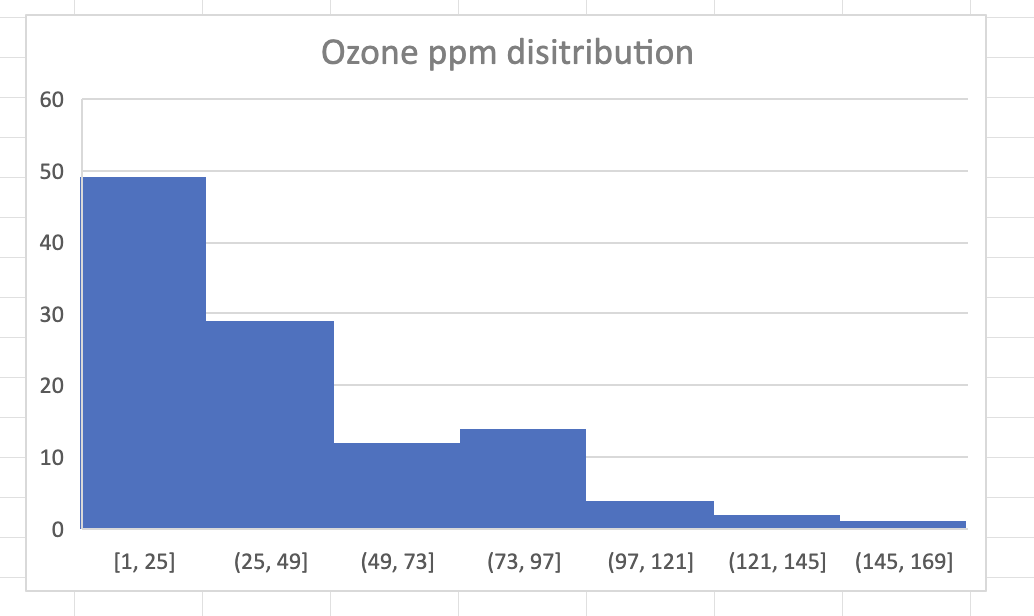
\includegraphics{./histogramozone.png}

\textbf{clean data}

First, from the data, we are going to clean the data, by removing those
that are have the value NA or not available.

1. Select all the data, and search for the filter.

2. Then, it will appear the drop down menu for each column, select the
drop down menu on the first column which is Ozone

3. Select NA. To remove it, select all from the row that has NA until
the bottom and select delete rows 6-151.

4. Select the drop down menu on column Ozone, select all and apply, it
will give back the table, however there's no NA anymore on the Ozone.

Looking at the data, there still some NA on the column B for Solar.R.
Repeat the way just like before. Next, to make it earlier to read the
data, sort the day and month to be in order. Select the column for
month, click the sort from smallest to largest, do the same for day.

\textbf{Scatter plot}

Using the air quality data sets, click on column A(ozone) and D
(temperature) to show the correlation between both of them. After
clicking on both column, I'm going to insert the scatter plot. The
scatter plot shows a relationship between Ozone levels (y-axis) and
Temperature (x-axis). The general trend indicates a positive
correlation: as the temperature increases, the ozone level tends to
increase as well.

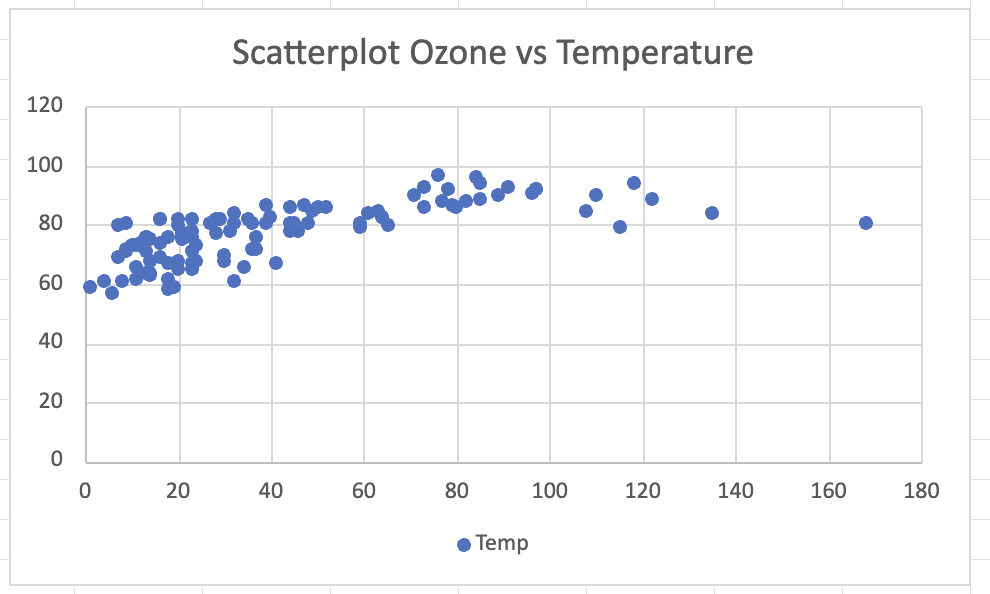
\includegraphics{./scatterplotozone.png}

\textbf{Pivot Table \& Chart}

To make a pivot table and chart, first select all the data, and click
insert. On the let corner, it will appear the pivot menu, press that and
select the create own pivot table. I select and drag ozone, temperature,
Solar. R, and Wind to the value, for the row I'll put only the month.
Then, I change the value field settings to average, this is to provide
the average of ozone, temperature, Solar. R, and Wind monthly. After
doing the pivot table, select that pivot table and insert the pivot
chart to create the visualization.

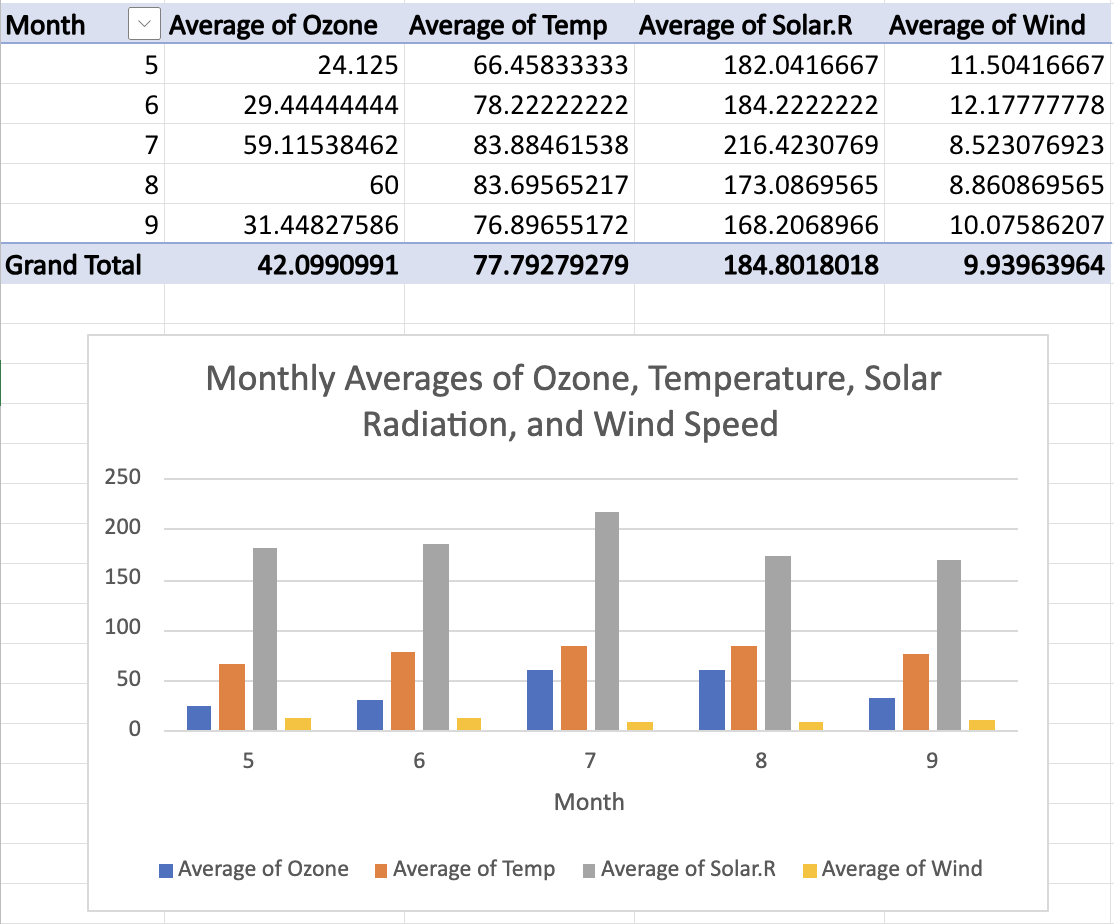
\includegraphics{./pivot1.png}

From the pivot table and chart above, it shows that ozone levels appear
to increase with higher temperature and solar radiation but decrease
with higher wind speeds.

Next, I'm going to provide another pivot table, that shows the average
of ozone, temperature, Solar. R, and Wind daily from day 1 to 31. To do
that, select again the first table, the one that was cleaned, then again
select the pivot table and choose the create own pivot table.

I select and drag ozone, temperature, Solar. R, and Wind to the value,
for the row I'll put only the day. Then, I change the value field
settings to average, this is to provide the average of ozone,
temperature, Solar. R, and Wind per day.

Now, I'm going to add the pivot chart from that new pivot table. I
choose two charts, from those two I can create conclusion and better
visualizations.

From the chart presented below, the average daily of Temperature and
Wind each have a positive correlation, however not with the average
daily of Solar. R and the Ozone. Also, on day 15 it shows the lowest
average of ozone and solar. r.

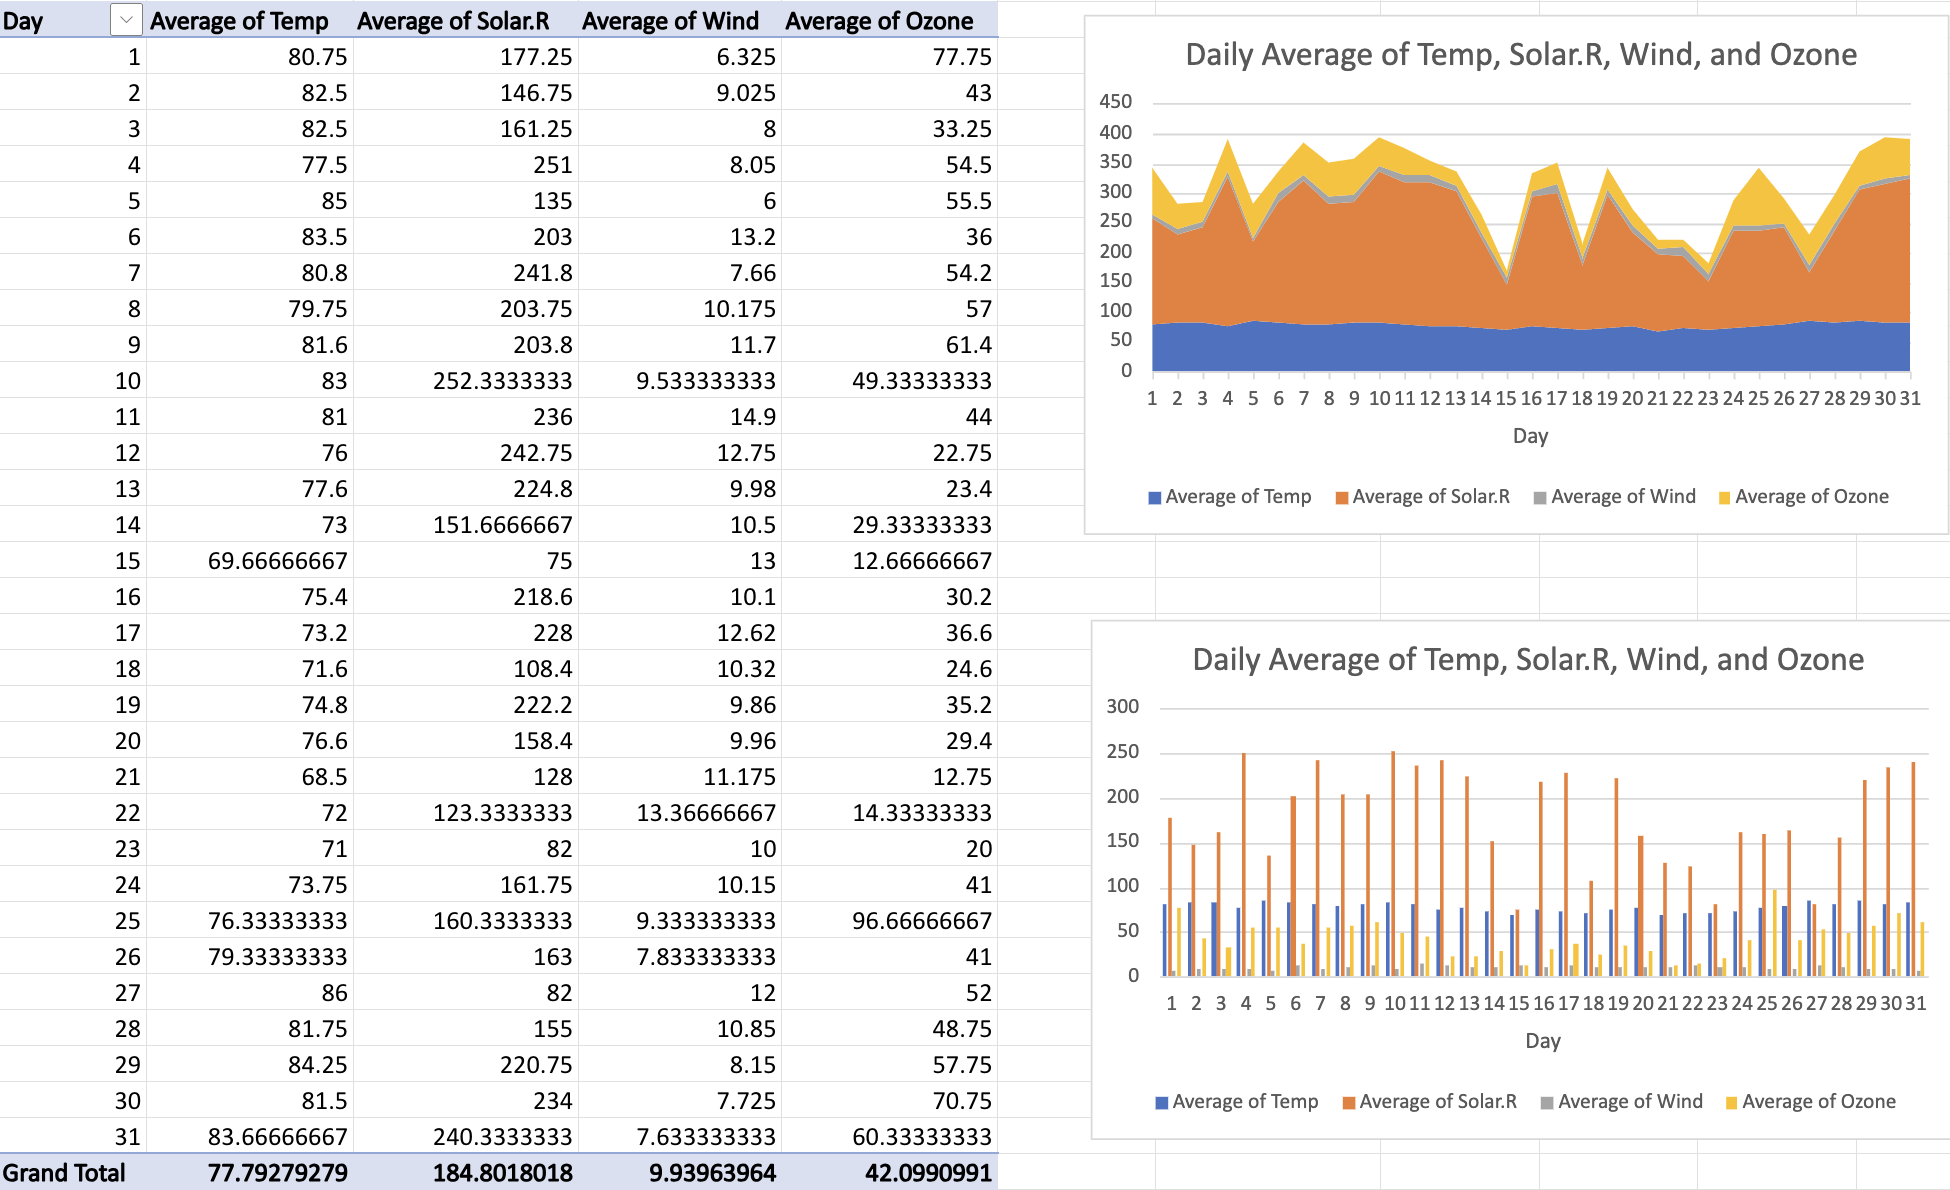
\includegraphics{./pivot2.png}

Third, I'm going to make another pivot table that can show more detailed
on each month per day.I'm going to choose to present the 5th month, so
I'm going to press the drop down menu from the column ``month'' and
select only the 5. Next, the table will only provide the information
from month 5, day 1-31 and the sum of ozone, wind, temp, and solar.r.

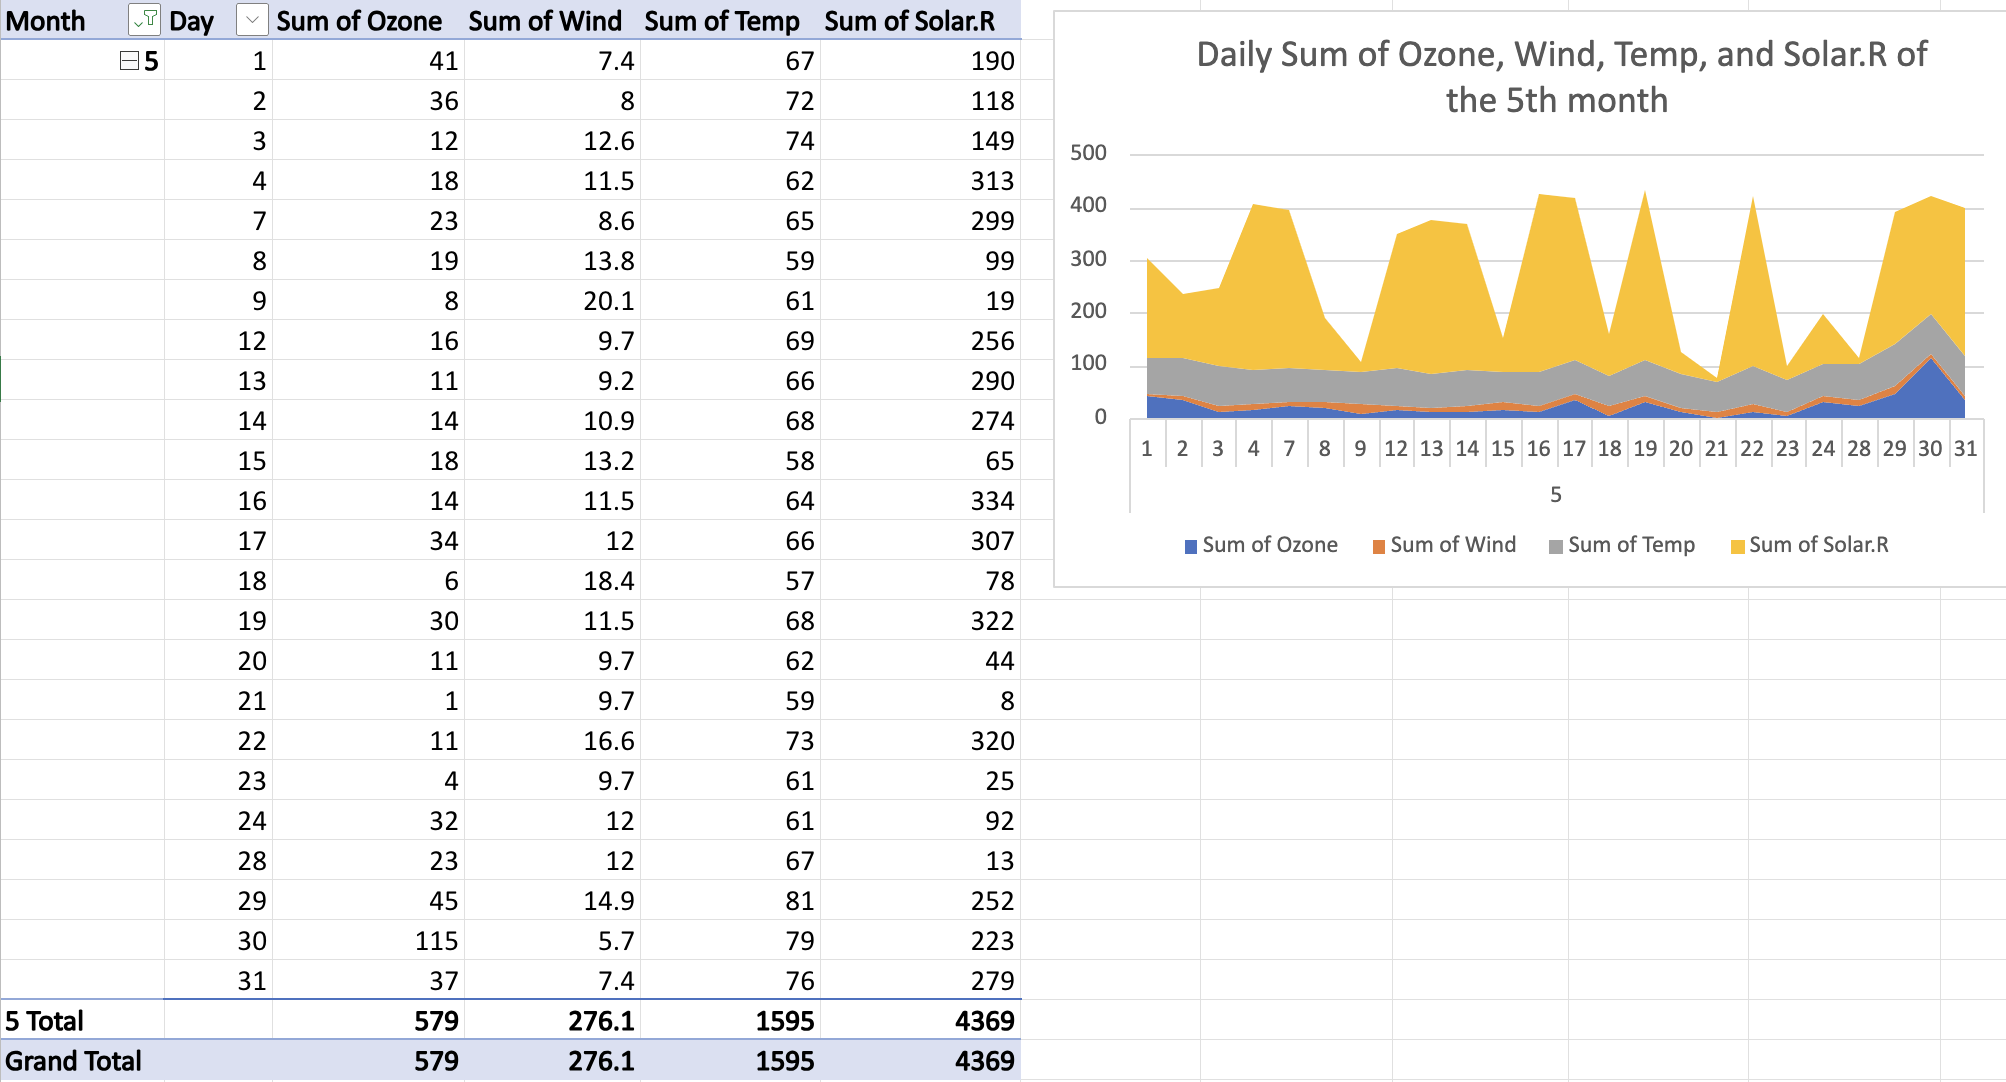
\includegraphics{./pivot3.png}

From the chart, we can see that, on day 30 from the 5th month, it shows
the highest sum of ozone.

\textbf{Individual Project}

** Who collected the data**

The source that I chose is National Transportation Library (NTL) Data.
There are lots of data sets from NTL, which can be access through
\url{https://ntl.bts.gov/ntl}. Data set that I chose is motor vehicle
safety. This data set is collected by U.S. Department of Transportation,
National Highway Traffic Safety Administration, National Center for
Statistics and Analysis, and Fatality Analysis Reporting System (FARS)
Database. I'm interested in this one, because it is critical to
understand trends in road safety, which is a major public concern. The
data that I collect is from this link
\url{https://www.bts.gov/content/motor-vehicle-safety-data}.

\textbf{Purpose}

Monitoring the trends in motor vehicle safety in the U.S., including
fatalities, injuries, and crashes. It serves to assess the effectiveness
of safety regulations, technology advancements, and policy interventions
over time. From the visualizations, it can improve the safety measures
and highlight the effectiveness of road safety interventions over the
years, making it highly valuable for assessing long-term changes in
traffic-related fatalities and injuries.

\textbf{Variables}

\begin{itemize}
\item
  Fatalities - total number of deaths from motor vehicle crashes
\item
  Injured persons - total number of people injured in motor vehicle
  accidents
\item
  Crashes - total number of motor vehicle crashes
\item
  Vehicles miles traveled - total number of miles driven by vehicles
\end{itemize}

\subsection{Week 3}\label{week-3}

\section{Friday}\label{friday}

\subsection{Week 1}\label{week-1-1}

\subsection{Week 2}\label{week-2-1}

\textbf{Histogram}

In week 2, data sets that I am using is air quality data set. After
cleaning the data set explained below, select all the data and insert
the histogram chart to create the visualization of the data. The
variables for the histogram chart is only the ozone. From the histogram,
it shows the distribution of the ozone, most of the ozone are 1 to 25
ppm.

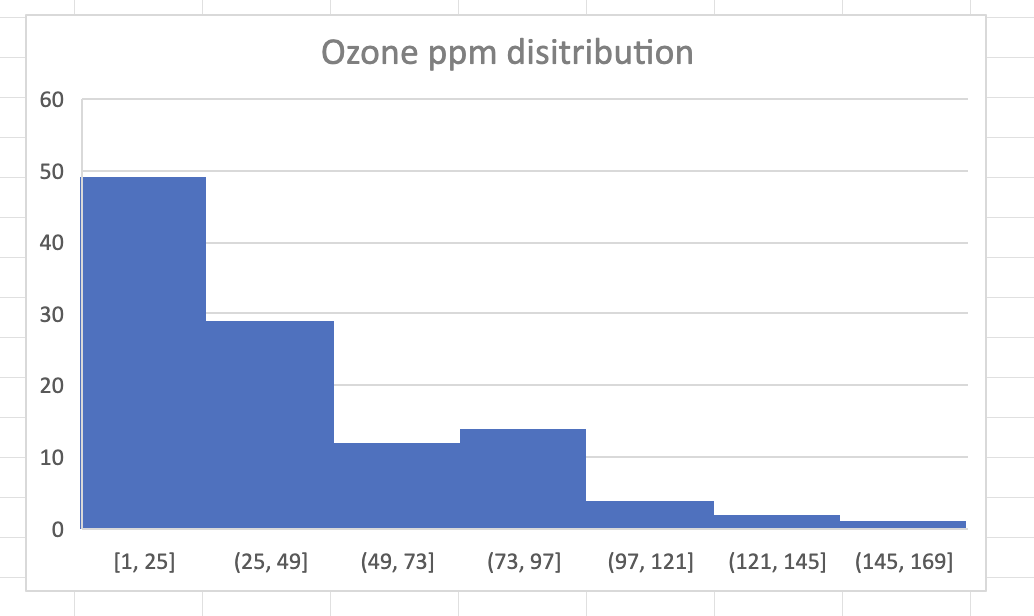
\includegraphics{./histogramozone.png}

\textbf{clean data}

First, from the data, we are going to clean the data, by removing those
that are have the value NA or not available.

1. Select all the data, and search for the filter.

2. Then, it will appear the drop down menu for each column, select the
drop down menu on the first column which is Ozone

3. Select NA. To remove it, select all from the row that has NA until
the bottom and select delete rows 6-151.

4. Select the drop down menu on column Ozone, select all and apply, it
will give back the table, however there's no NA anymore on the Ozone.

Looking at the data, there still some NA on the column B for Solar.R.
Repeat the way just like before. Next, to make it earlier to read the
data, sort the day and month to be in order. Select the column for
month, click the sort from smallest to largest, do the same for day.

\textbf{Scatter plot}

Using the air quality data sets, click on column A(ozone) and D
(temperature) to show the correlation between both of them. After
clicking on both column, I'm going to insert the scatter plot. The
scatter plot shows a relationship between Ozone levels (y-axis) and
Temperature (x-axis). The general trend indicates a positive
correlation: as the temperature increases, the ozone level tends to
increase as well.

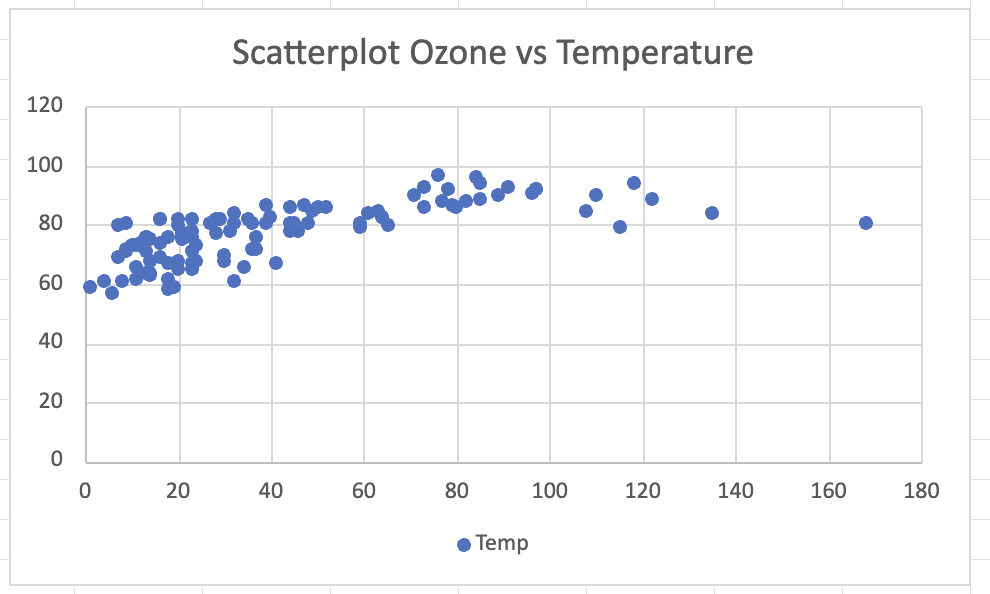
\includegraphics{./scatterplotozone.png}

\textbf{Pivot Table \& Chart}

To make a pivot table and chart, first select all the data, and click
insert. On the let corner, it will appear the pivot menu, press that and
select the create own pivot table. I select and drag ozone, temperature,
Solar. R, and Wind to the value, for the row I'll put only the month.
Then, I change the value field settings to average, this is to provide
the average of ozone, temperature, Solar. R, and Wind monthly. After
doing the pivot table, select that pivot table and insert the pivot
chart to create the visualization.

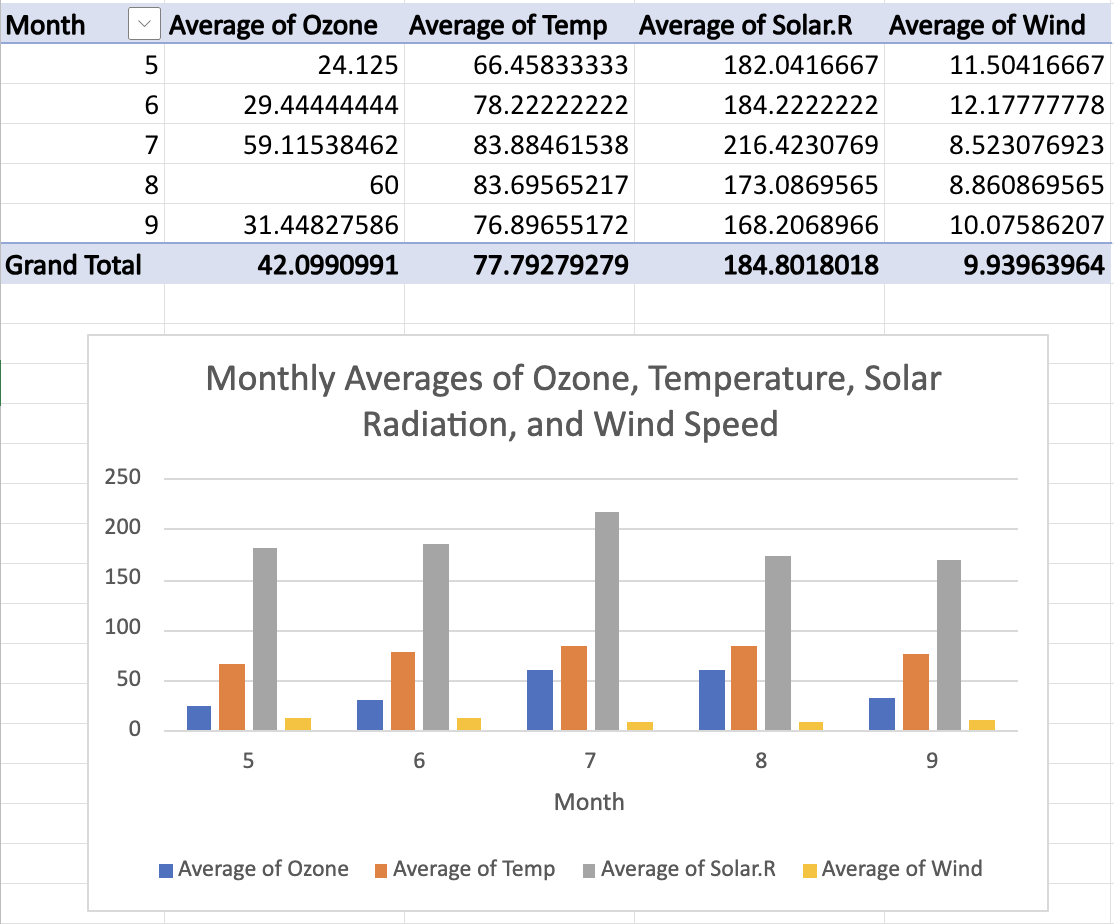
\includegraphics{./pivot1.png}

From the pivot table and chart above, it shows that ozone levels appear
to increase with higher temperature and solar radiation but decrease
with higher wind speeds.

Next, I'm going to provide another pivot table, that shows the average
of ozone, temperature, Solar. R, and Wind daily from day 1 to 31. To do
that, select again the first table, the one that was cleaned, then again
select the pivot table and choose the create own pivot table.

I select and drag ozone, temperature, Solar. R, and Wind to the value,
for the row I'll put only the day. Then, I change the value field
settings to average, this is to provide the average of ozone,
temperature, Solar. R, and Wind per day.

Now, I'm going to add the pivot chart from that new pivot table. I
choose two charts, from those two I can create conclusion and better
visualizations.

From the chart presented below, the average daily of Temperature and
Wind each have a positive correlation, however not with the average
daily of Solar. R and the Ozone. Also, on day 15 it shows the lowest
average of ozone and solar. r.

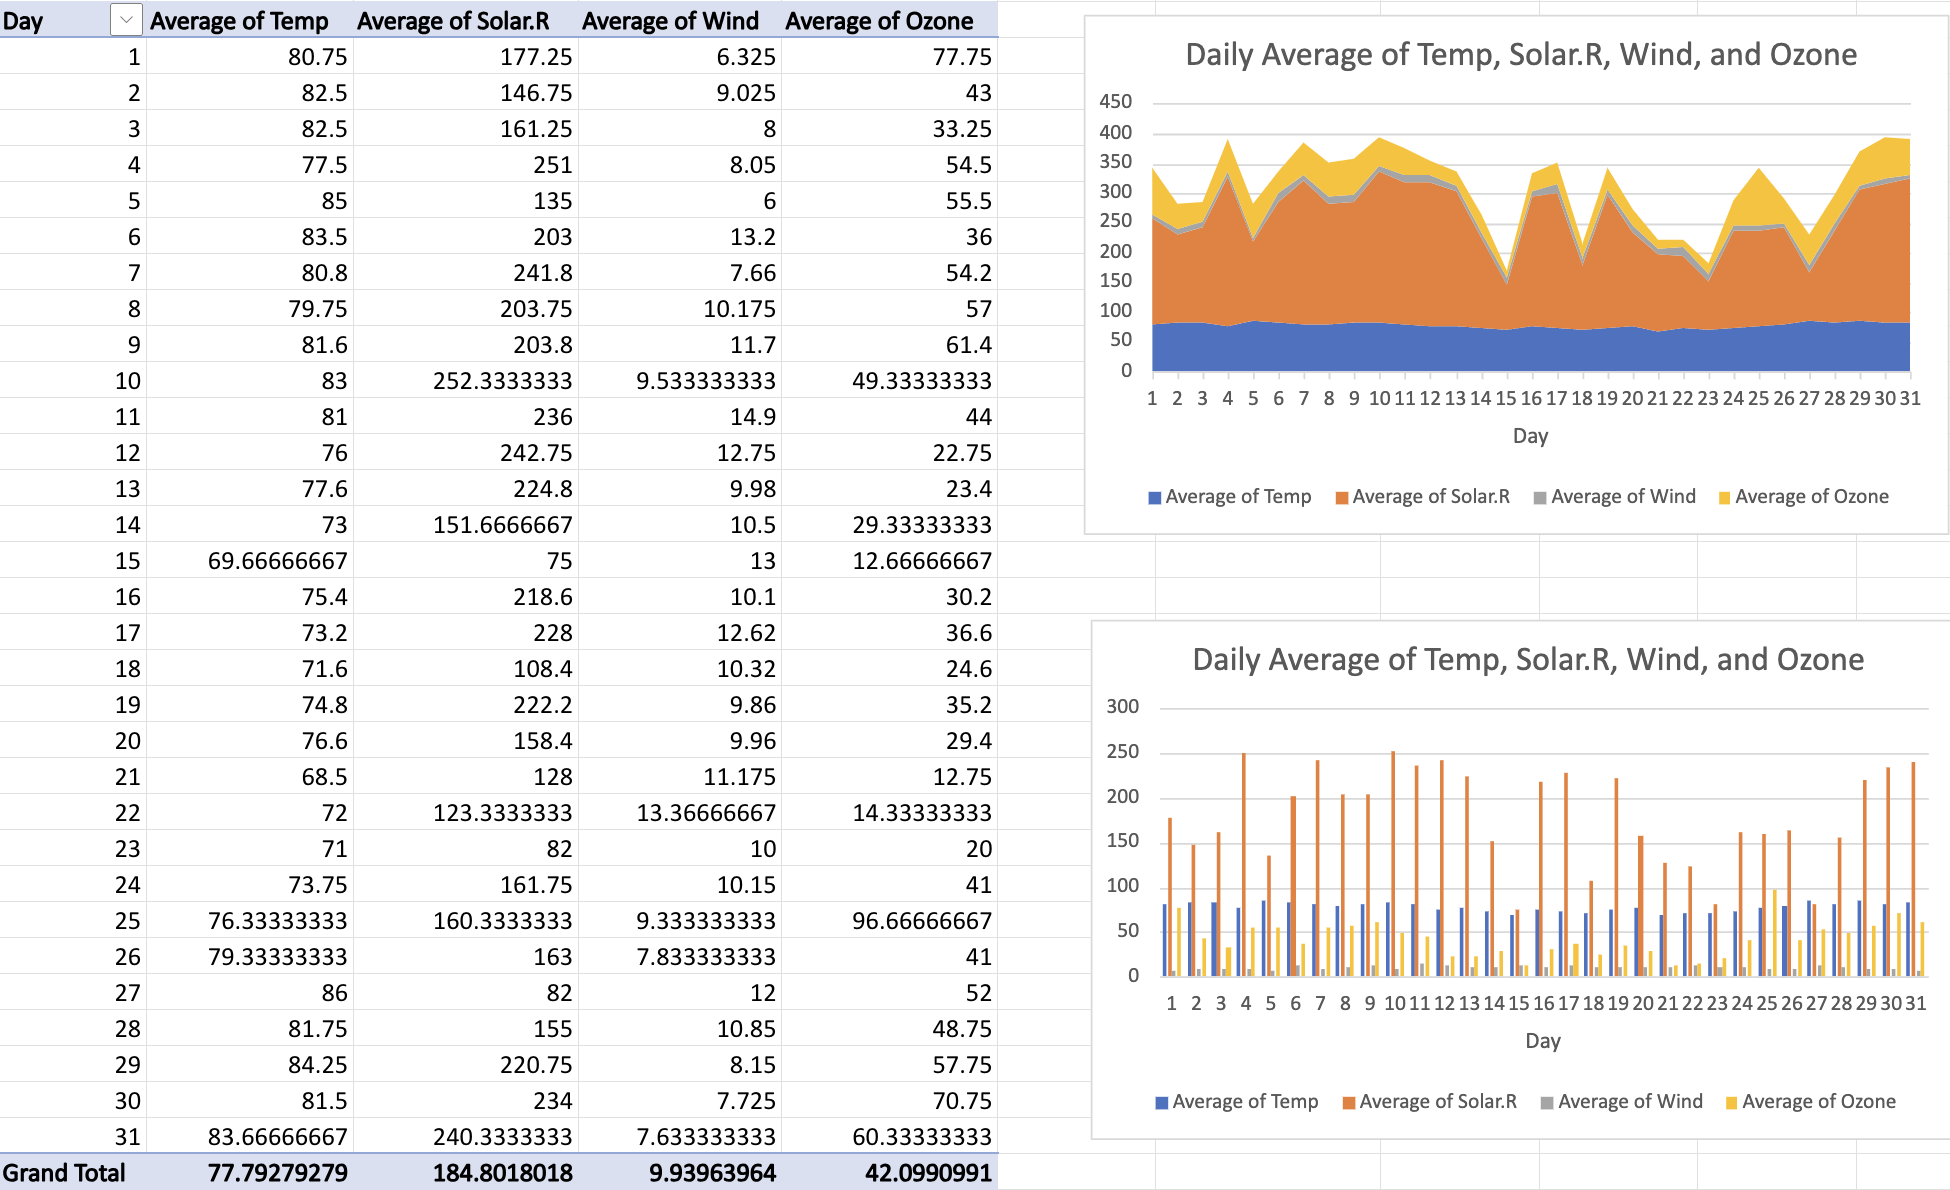
\includegraphics{./pivot2.png}

Third, I'm going to make another pivot table that can show more detailed
on each month per day.I'm going to choose to present the 5th month, so
I'm going to press the drop down menu from the column ``month'' and
select only the 5. Next, the table will only provide the information
from month 5, day 1-31 and the sum of ozone, wind, temp, and solar.r.

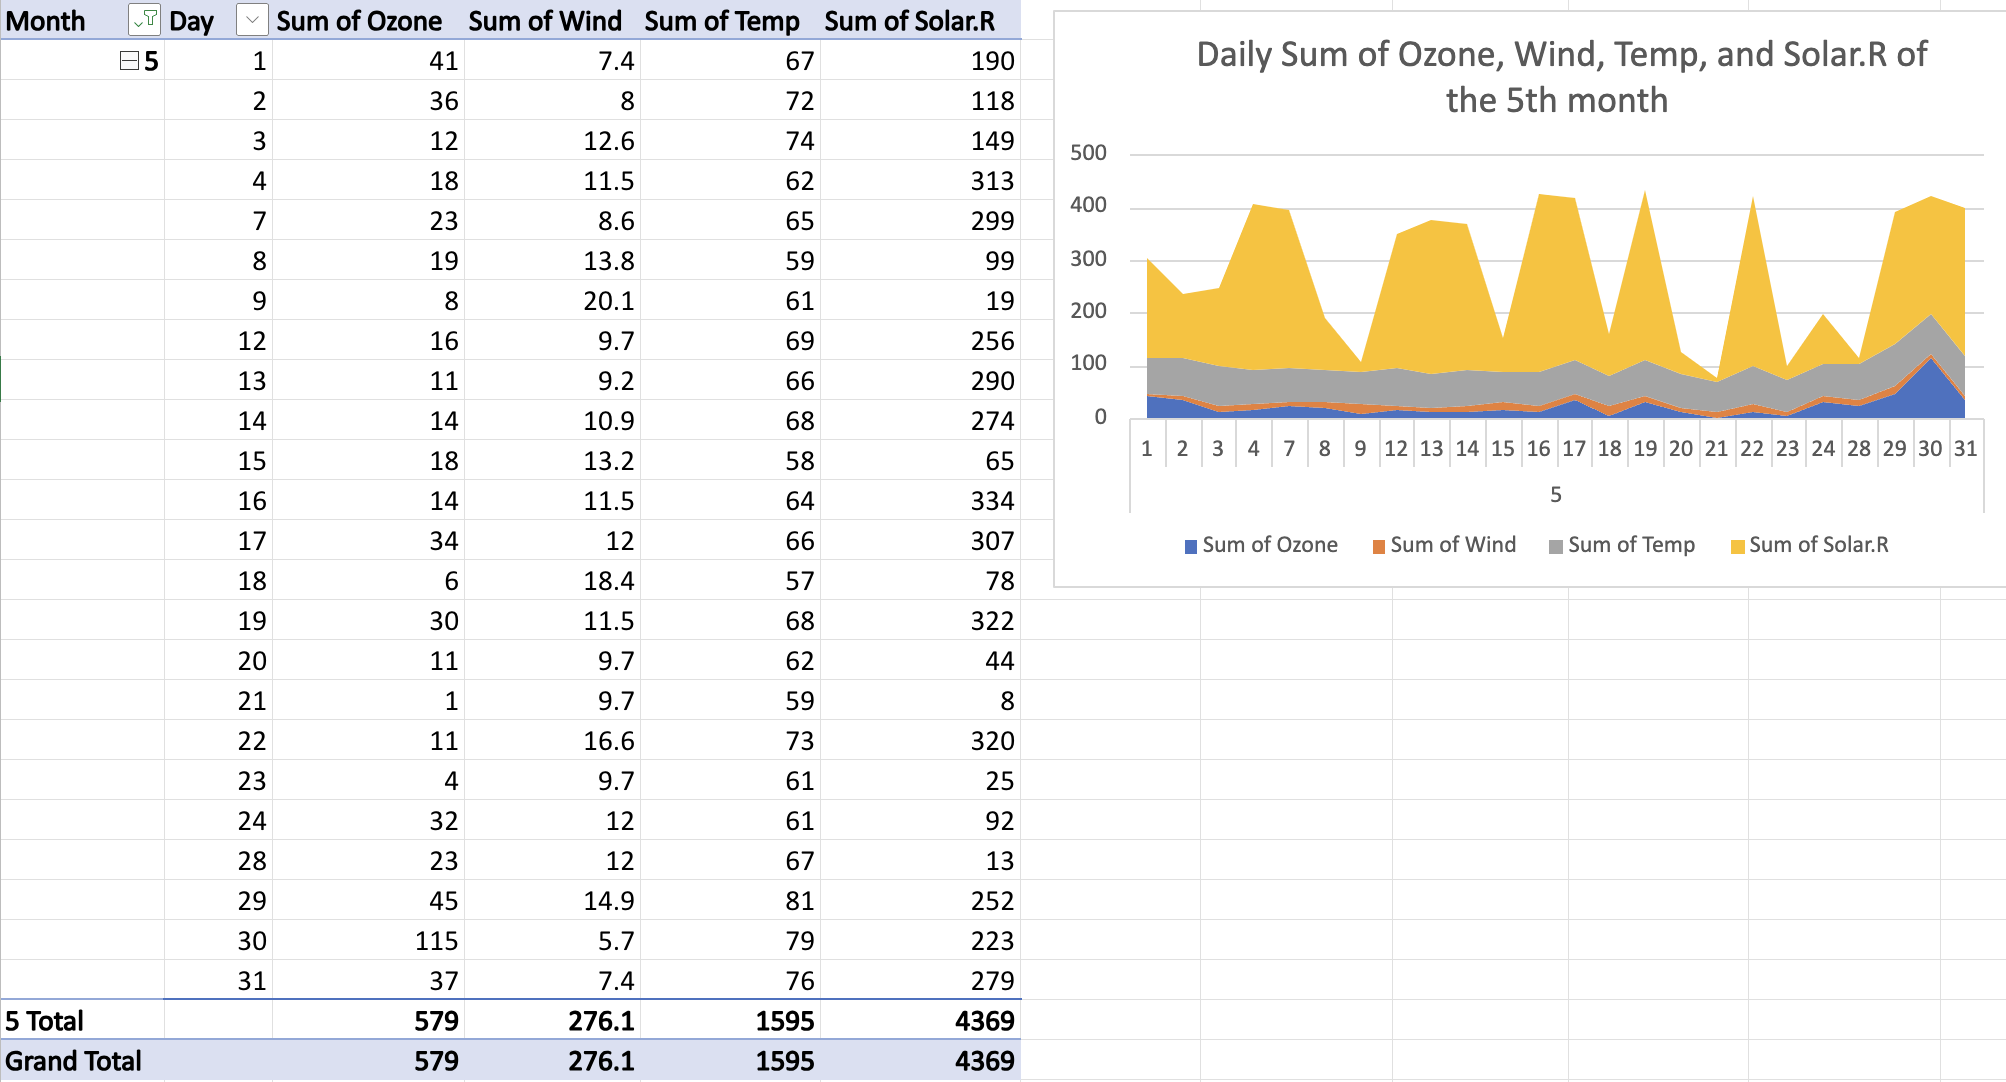
\includegraphics{./pivot3.png}

From the chart, we can see that, on day 30 from the 5th month, it shows
the highest sum of ozone.

\textbf{Individual Project}

\textbf{Who collected the data}

The source that I chose is National Transportation Library (NTL) Data.
There are lots of data sets from NTL, which can be access through
\url{https://ntl.bts.gov/ntl}. Data set that I chose is motor vehicle
safety. This data set is collected by U.S. Department of Transportation,
National Highway Traffic Safety Administration, National Center for
Statistics and Analysis, and Fatality Analysis Reporting System (FARS)
Database. I'm interested in this one, because it is critical to
understand trends in road safety, which is a major public concern. The
data that I collect is from this link
\url{https://www.bts.gov/content/motor-vehicle-safety-data}.

\textbf{Purpose}

Monitoring the trends in motor vehicle safety in the U.S., including
fatalities, injuries, and crashes. It serves to assess the effectiveness
of safety regulations, technology advancements, and policy interventions
over time. From the visualizations, it can improve the safety measures
and highlight the effectiveness of road safety interventions over the
years, making it highly valuable for assessing long-term changes in
traffic-related fatalities and injuries.

\textbf{Variables}

\begin{itemize}
\item
  Fatalities - total number of deaths from motor vehicle crashes
\item
  Injured persons - total number of people injured in motor vehicle
  accidents
\item
  Crashes - total number of motor vehicle crashes
\item
  Vehicles miles traveled - total number of miles driven by vehicles
\end{itemize}

\subsection{Week 3}\label{week-3-1}

\section{Midterm Project}\label{midterm-project}

\subsection{Week 1}\label{week-1-2}

\subsection{Week 2}\label{week-2-2}

\subsection{Week 3}\label{week-3-2}

\href{introduction.html}{Back to Main Page}

\bookmarksetup{startatroot}

\chapter{Caleb Pena}\label{caleb-pena}

This page contains all of Caleb Pena's submissions this semester
organized into different sections.

\section{Wednesday}\label{wednesday-1}

\subsection{Week 1}\label{week-1-3}

\subsection{Week 2}\label{week-2-3}

\textbf{Wednesday, September 4, 2024}

I am using the airquality dataset, which is a collection of data
collected from 153 observations based on 6 different variables. These
variables include:

Ozone (Numeric) - Mean ozone in parts per billion from 1300 to 1500
hours at Roosevelt Island

Solar R (Numeric) - Solar radiation in Langleys in the frequency band
4000--7700 Angstroms from 0800 to 1200 hours at Central Park

Wind (Numeric) - Average wind speed in miles per hour at 0700 and 1000
hours at LaGuardia Airport

Temp (Numeric) - Maximum daily temperature in degrees Fahrenheit at La
Guardia Airport

Month (Numeric) - Months from May to September

Day (Numeric) - Days of the months ranging from 1 to 31

I am using Excel to clean the data, which removes all the rows which
have N/A values, and I did an exploration analysis.

\textbf{Ozone vs Temperature Histogram}

This histogram represents the amount of temperature values calculated
within each border of values of ozone. For example, in the range of
ozone level between 1 and 25, there were 49 temperature values recorded.

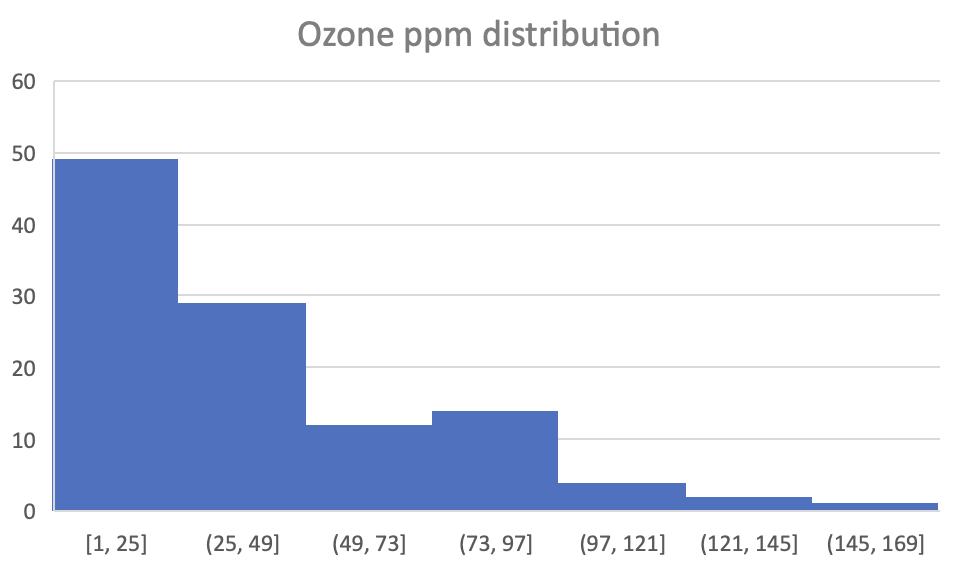
\includegraphics{Hist_Ozone_Pena.png}

\textbf{Ozone vs Temperature Scatter Plot}

This scatter plot displays the correlation between the ozone levels and
the temperature values recorded within these five months. As the ozone
level increased, so did the temperature value, with one outlier.

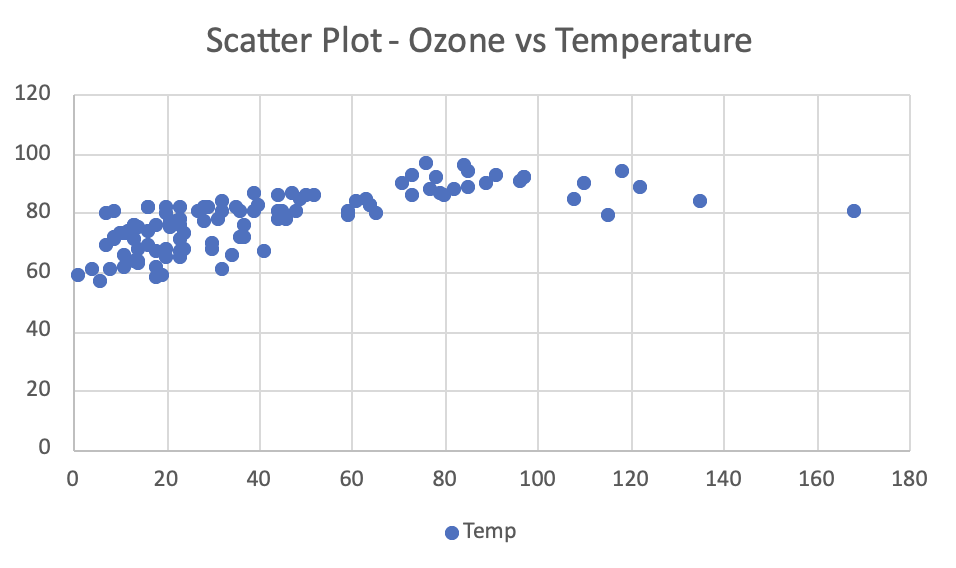
\includegraphics{Scat_Oz_Temp_Pena.png}

\textbf{My First PivotTable}

This PivotTable displays the average values of each variable for each of
the five months.

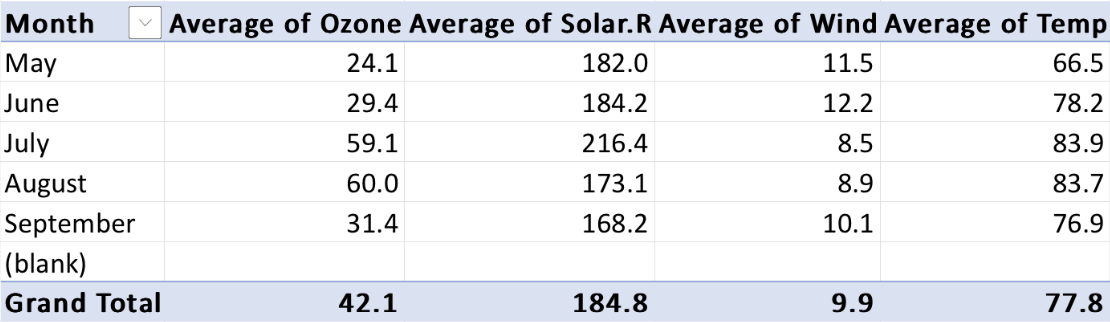
\includegraphics{PivotTable1_Summary_Variables_Pena.png}

\textbf{My Second PivotTable}

This PivotTable displays the average temperature values for each day of
each month.

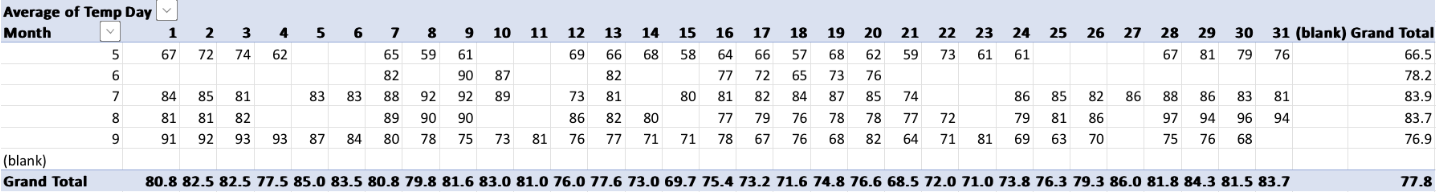
\includegraphics{PivotTable2_Average_Temp_Pena.png}

\subsection{Week 3}\label{week-3-3}

\section{Friday}\label{friday-1}

\subsection{Week 1}\label{week-1-4}

\subsection{Week 2}\label{week-2-4}

\textbf{Friday, September 6, 2024}

Using the same airquality datasets, I worked on creating PivotCharts
from previous and new PivotTables comparing different values and
variables.

\textbf{PivotChart1 - Average Variable Values by `Month'}

This pivot table produced this chart. These are the average values of
each variables for each of the five months. The PivotChart shows the
comparison between each of the variables and how each one increases or
decreases throughout the five months.

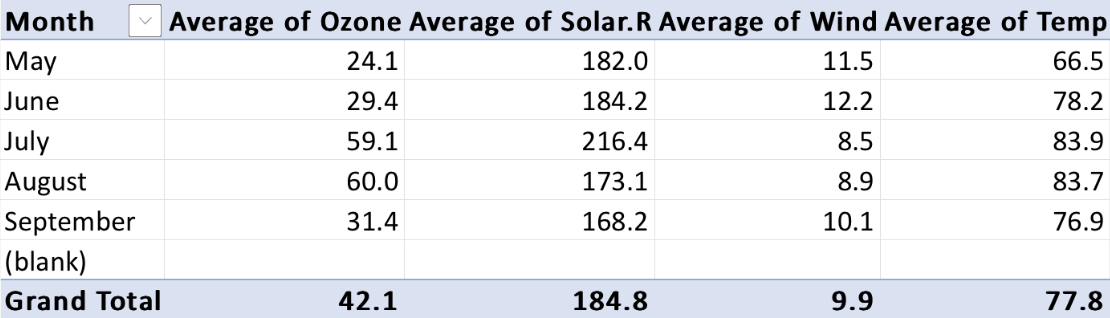
\includegraphics{PivotTable1_AverageVariableValues_Pena.png}

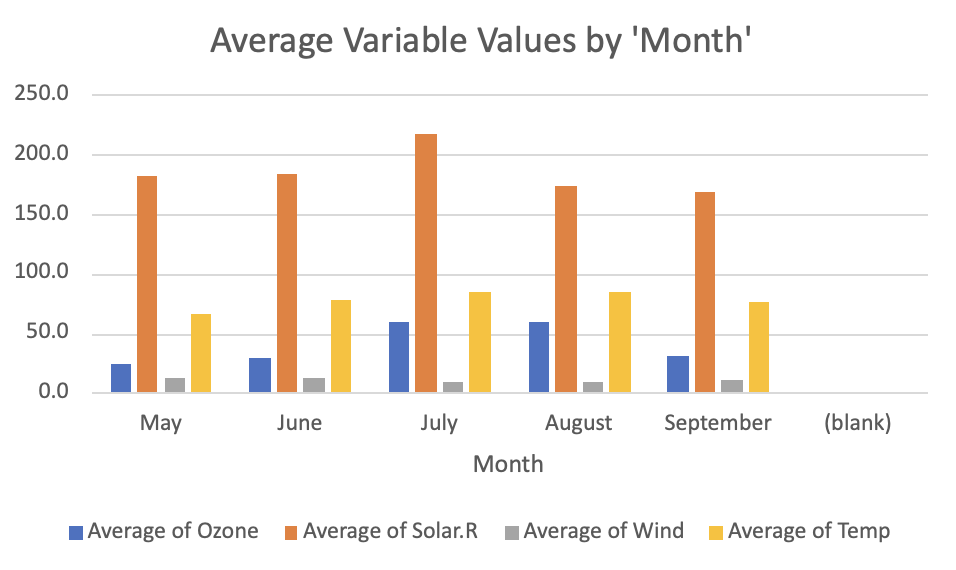
\includegraphics{PivotChart1_AverageVariableValues_Pena.png}

\textbf{PivotChart2 - Average Ozone Values by `Temp'}

This pivot table produced this chart. This PivotChart displays the
average ozone values for each temperature value that was recorded. As
the temperature values increase, the average values for the ozone can be
seen to also increase in a correlated way.

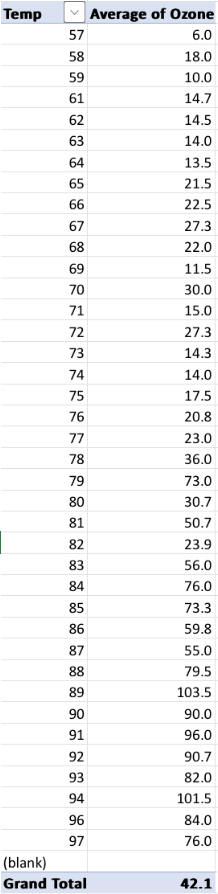
\includegraphics{PivotTable2_AverageOzoneByTemp_Pena.png}

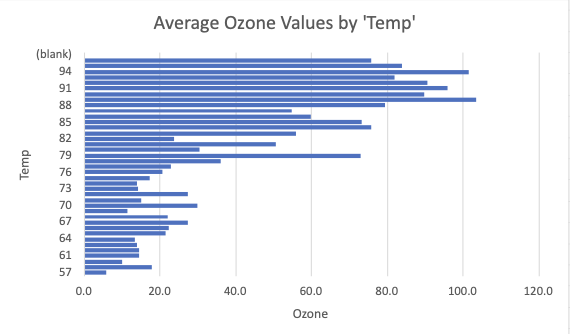
\includegraphics{PivotChart2_AverageOzoneByTemp_Pena.png}

\textbf{PivotChart3 - Average Temp and Ozone Values by `Wind'}

This pivot table produced this chart. This PivotChart displays the
average values of both temperature and ozone for each wind value
recorded. From the chart, it is evident that as the wind values
increase, the average values for temperature seem to slightly decrease
and the average values for the ozone levels seem to greatly decrease.

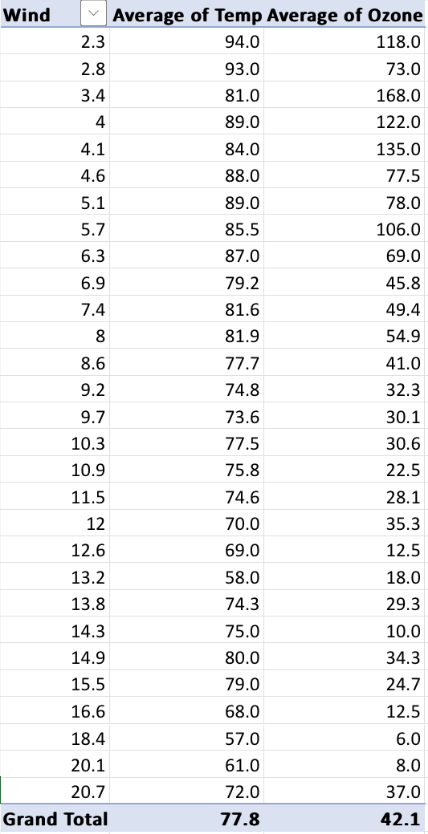
\includegraphics{PivotTable3_AverTempOzoneByWind_Pena.png}

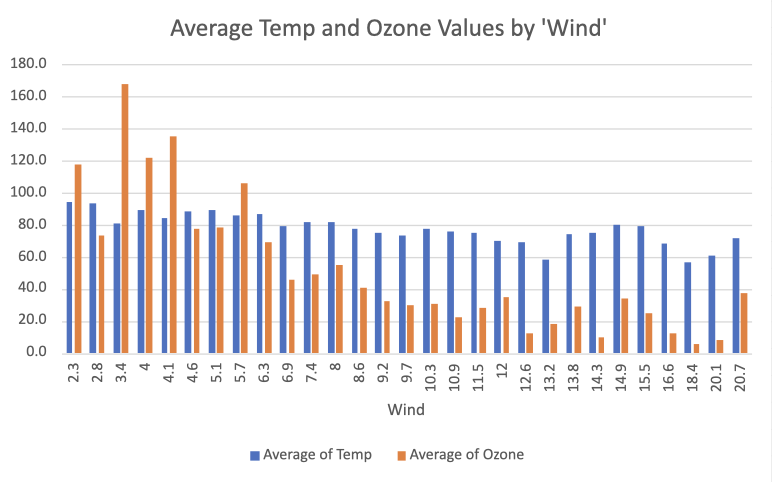
\includegraphics{PivotChart3_AverTempOzoneByWind_Pena.png}

\textbf{Newport Oregon Oceanographic Temperature Dataset}

Starting off in the year 1996, a group of NOAA Fisheries and Oregon
State University Scientists sampled the Newport Hydrographic Line
fortnightly to understand changing ocean conditions. The various
variable data was collected from a station located 5 miles off the coast
of Newport, Oregon. The scientists sampled and collected data regarding
seven different variables:

Day (Numerical) - The specific day of the month in which the data was
sampled.

Month (Numerical) - The specific month of the year in which the data was
sampled.

Year (Numerical) - The specific year in which the data was sampled.

Temperature (Numerical) - Oceanographic, temperature data collected from
a 50 m water depth.

Oxygen (Numerical) - Oceanographic, oxygen data collected from a 50 m
water depth.

Northern Copepod Biomass (Numerical) - Copepod community data collected
from from vertical net samples on the northern area

Southern Copepod Biomass (Numerical) - Copepod community data collected
from from vertical net samples on the southern area

\textbf{Visualizations}

The descriptive statistics of all the water temperatures sampled
throughout the 28 years. The average temperature of all collective 28
years is 8.75 ºC. The lowest temperature recorded of all 28 years is
6.92 ºC and the highest temperature recorded from all 28 years is 14.65
ºC.

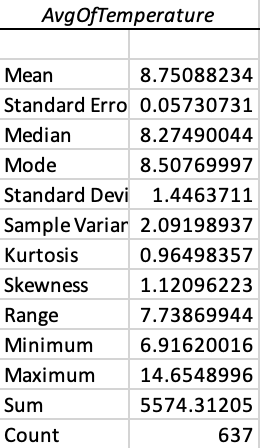
\includegraphics{TemperatureStats.png}

The peak temperatures of the water during the winter have a higher
average than the peak temperatures of the water during the summer.

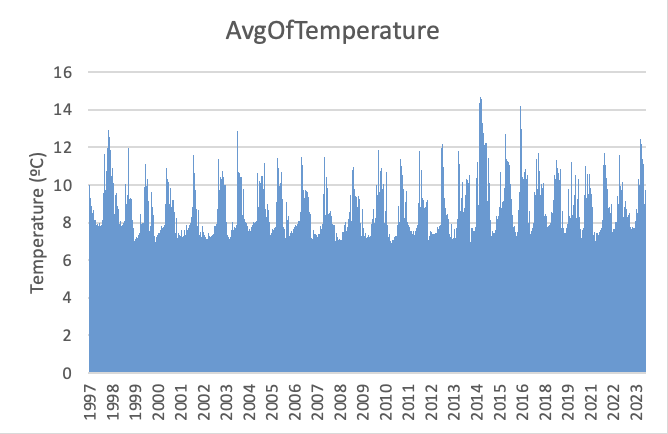
\includegraphics{TemperatureData.png}

Through the dot plot, the average of the temperatures is 8.75 ºC as most
of the dot population is visible there.

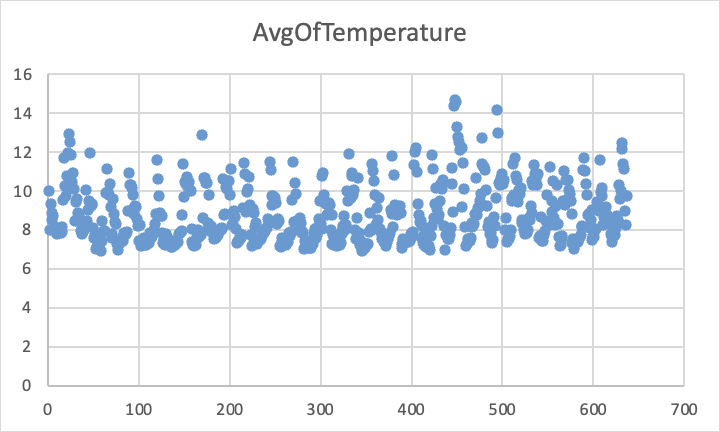
\includegraphics{TemperatureAverage.png}

The average temperatures of all collective 28 years gathered within each
month. During the summer months, the averages are lower. During the
winter months, the averages are higher.

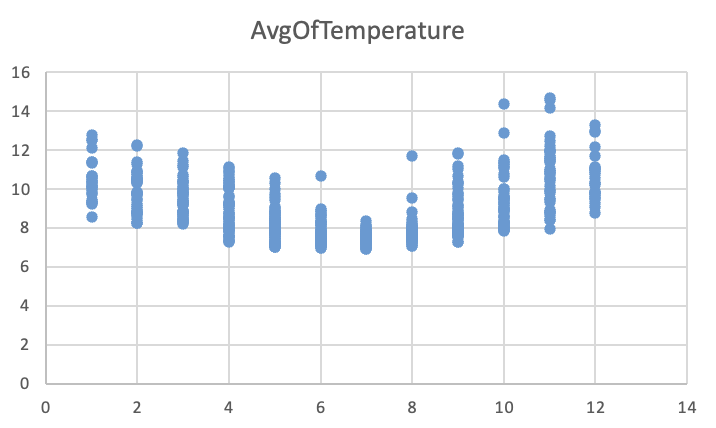
\includegraphics{TemperatureMonthAverage.png} \#\#\# Week 3

\section{Midterm Project}\label{midterm-project-1}

\subsection{Week 1}\label{week-1-5}

\subsection{Week 2}\label{week-2-5}

\subsection{Week 3}\label{week-3-4}

\href{introduction.html}{Back to Main Page}

\bookmarksetup{startatroot}

\chapter{Derrick Baruga}\label{derrick-baruga}

This page contains all of Derrick Baruga's submissions this semester
organized into different sections.

\section{Wednesday}\label{wednesday-2}

\subsection{Week 1}\label{week-1-6}

\subsection{Week 2}\label{week-2-6}

I am using the air-quality dataset, which contains air quality
measurements collected over several months, specifically from May to
September. The dataset includes the following variables: \textbf{Ozone},
\textbf{Solar.R} (solar radiation), \textbf{Wind} (wind speed in miles
per hour), \textbf{Temp} (temperature in degrees Fahrenheit),
\textbf{Month} (ranging from 5 for May to 9 for September), and
\textbf{Day} (ranging from 1 to 31).

\textbf{Cleaning The Data}

I used Excel to clean the data by removing all rows with NA values and
performed an exploratory analysis to identify patterns, trends, and
potential relationships between these variables over the specified
months and days.

\textbf{Ozone Histogram}

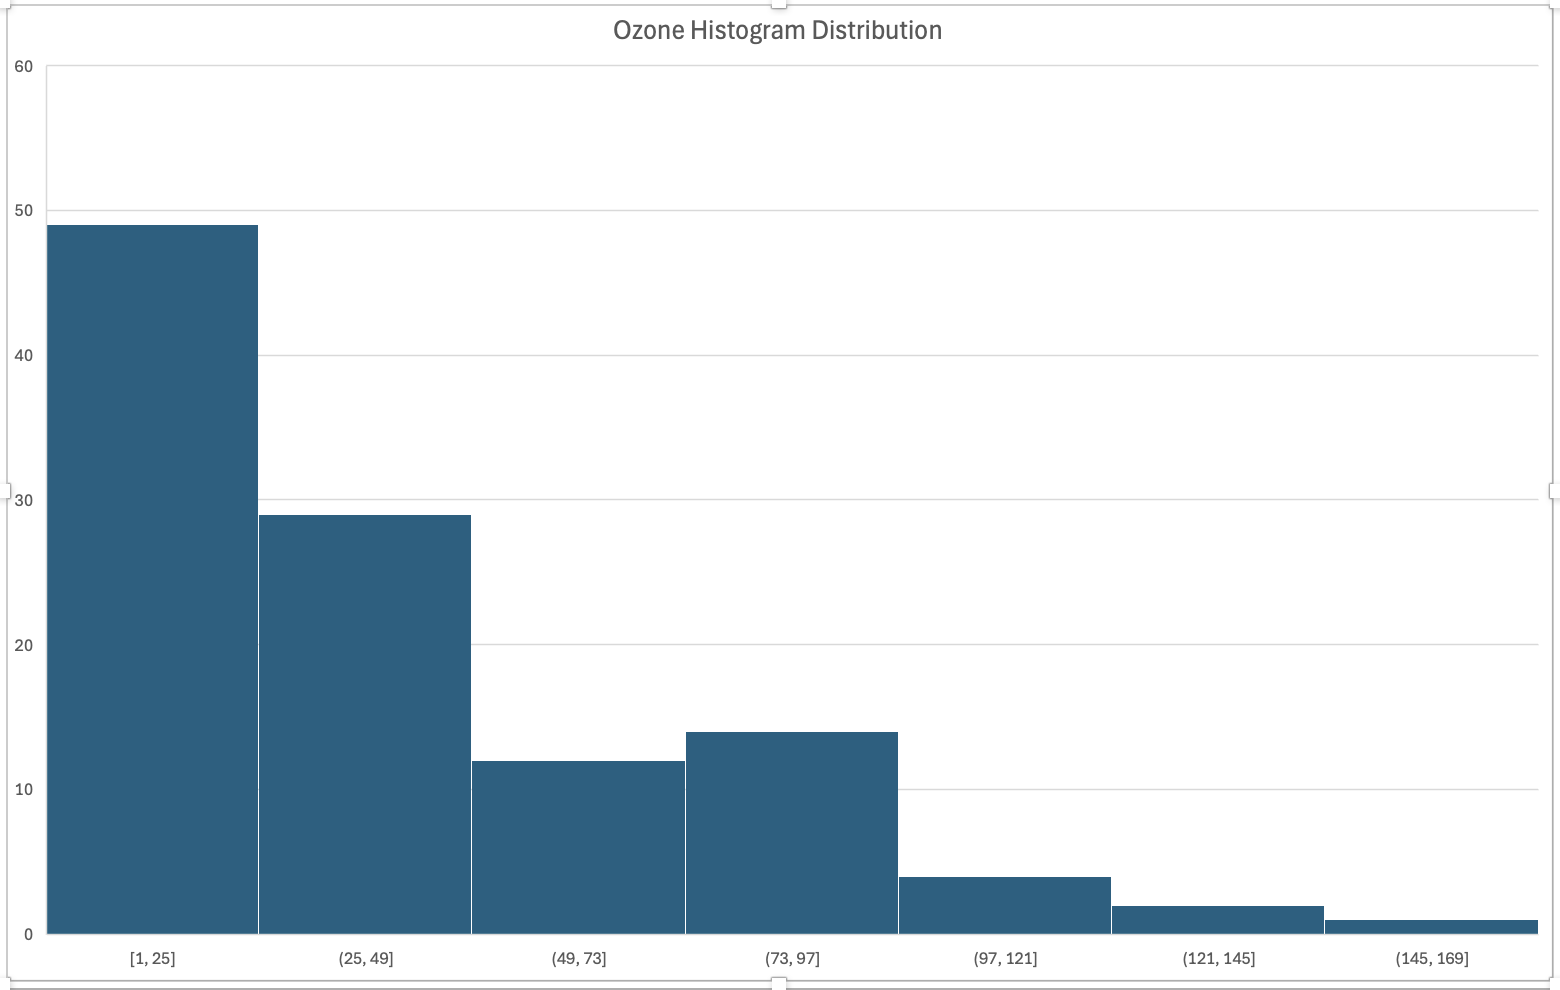
\includegraphics{hist_ozone_baruga.png}

The Ozone histogram has its highest values on the left and then curbs
off to the right, it indicates a right-skewed distribution.

This means:

\begin{itemize}
\tightlist
\item
  Most ozone values are low, with a few much higher values creating a
  long tail on the right.
\item
  The skewness could result from natural variability, pollution events,
  or weather conditions affecting ozone levels.
\end{itemize}

\textbf{Scatter Plot Ozone vs Temperature}

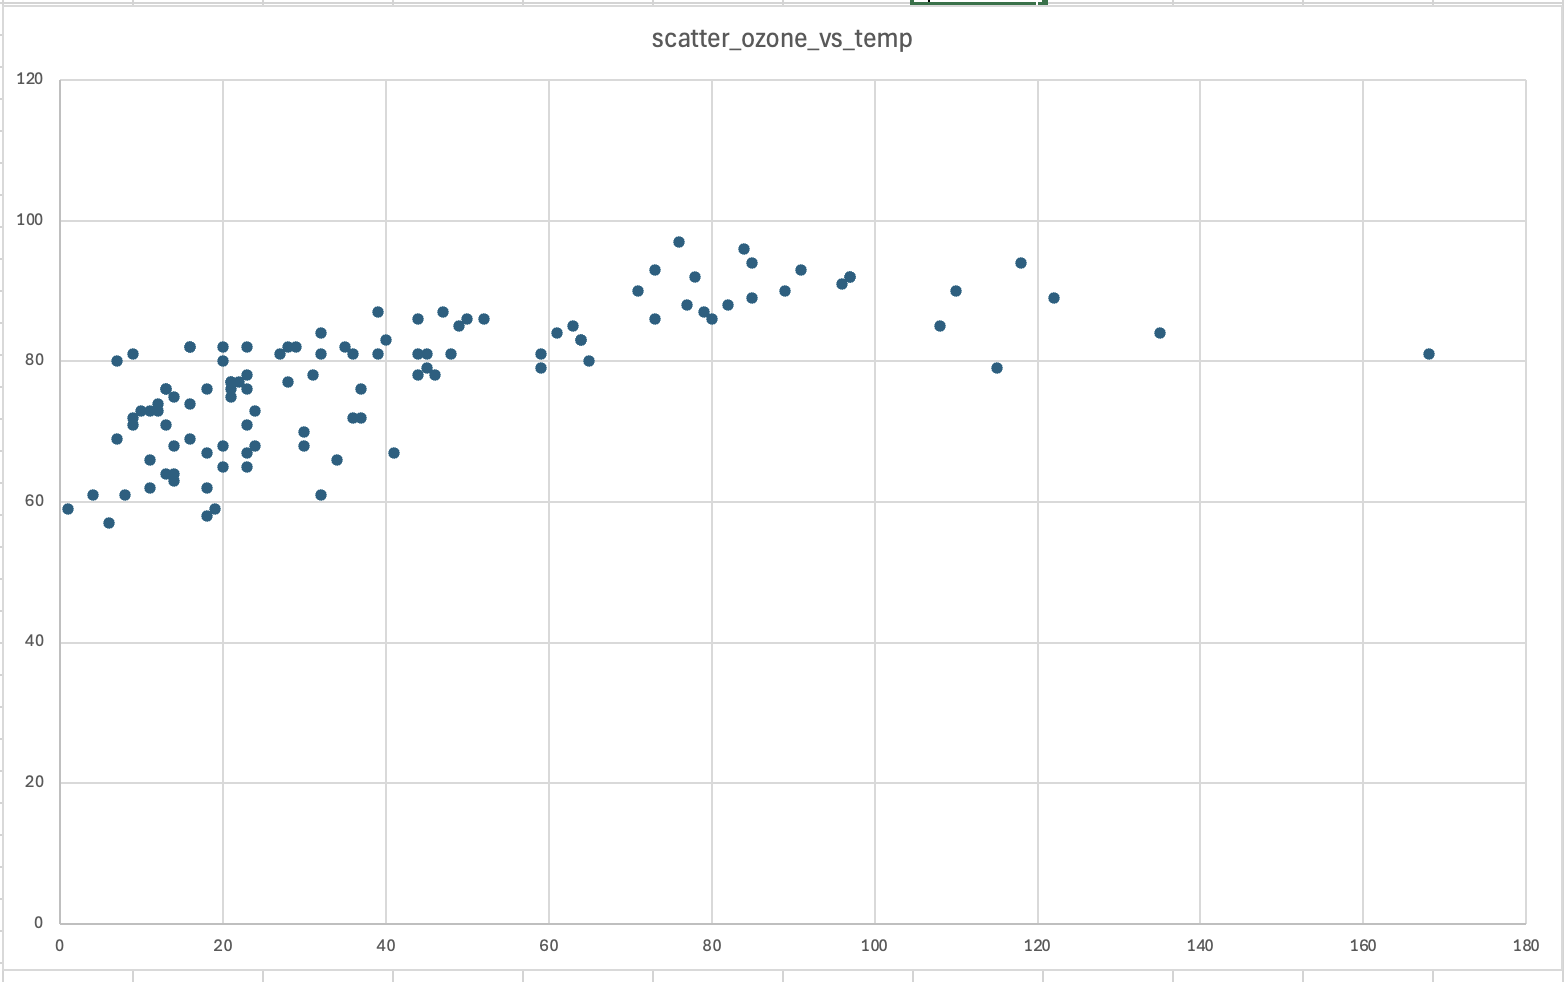
\includegraphics{scatter_ozone_vs_temp_baruga.png}

\begin{itemize}
\tightlist
\item
  A scatter plot of ozone (x-axis) vs.~temperature (y-axis) with a
  slight positive correlation means that higher ozone levels tend to be
  associated with higher temperatures. However, the relationship is
  weak, suggesting other factors (like wind, humidity, or pollution)
  also affect ozone levels and temperature.
\end{itemize}

\textbf{Pivot Table Average Ozones Per Day \& Month (Redacted)}

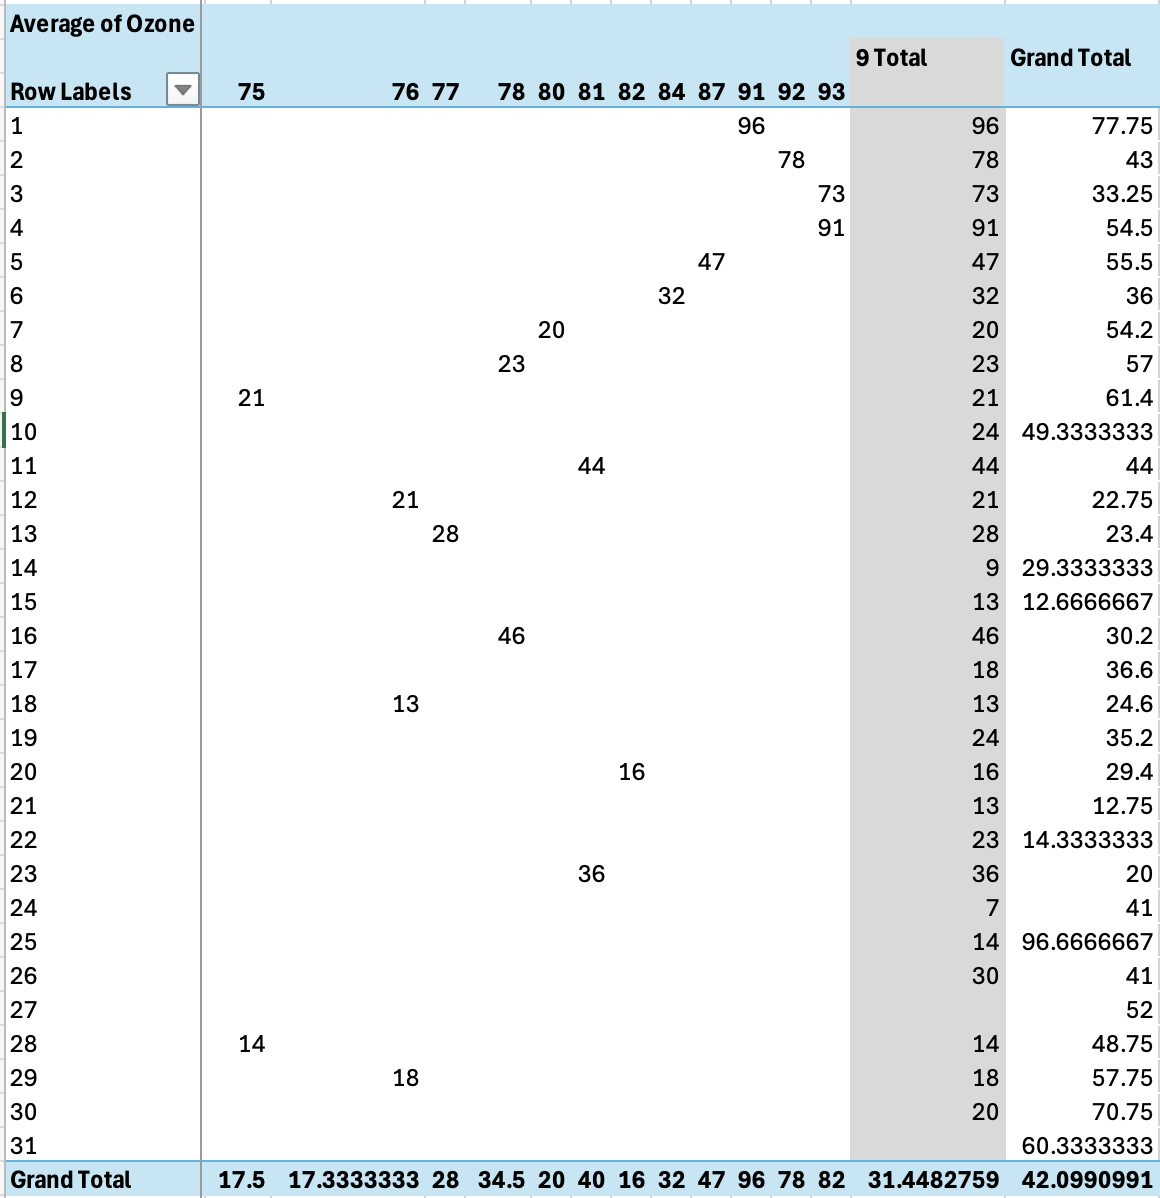
\includegraphics{pivot4_table_baruga.png}

\begin{itemize}
\tightlist
\item
  The pivot table presents daily sums for multiple variables
  (Temperature, Wind, Solar Radiation, and Ozone) over several months
  (May to September). The days with the highest ozone averages are Day
  25 in May (with an Ozone value of 5-65) and July (with an Ozone value
  of 7-74), with other notable days being Day 29 and Day 30 in May. The
  months with the highest ozone levels are May, which shows several days
  with high averages, and July, particularly on Days 25 and 29.
\end{itemize}

\textbf{Pivot Chart Average Ozones Per Day \& Month}

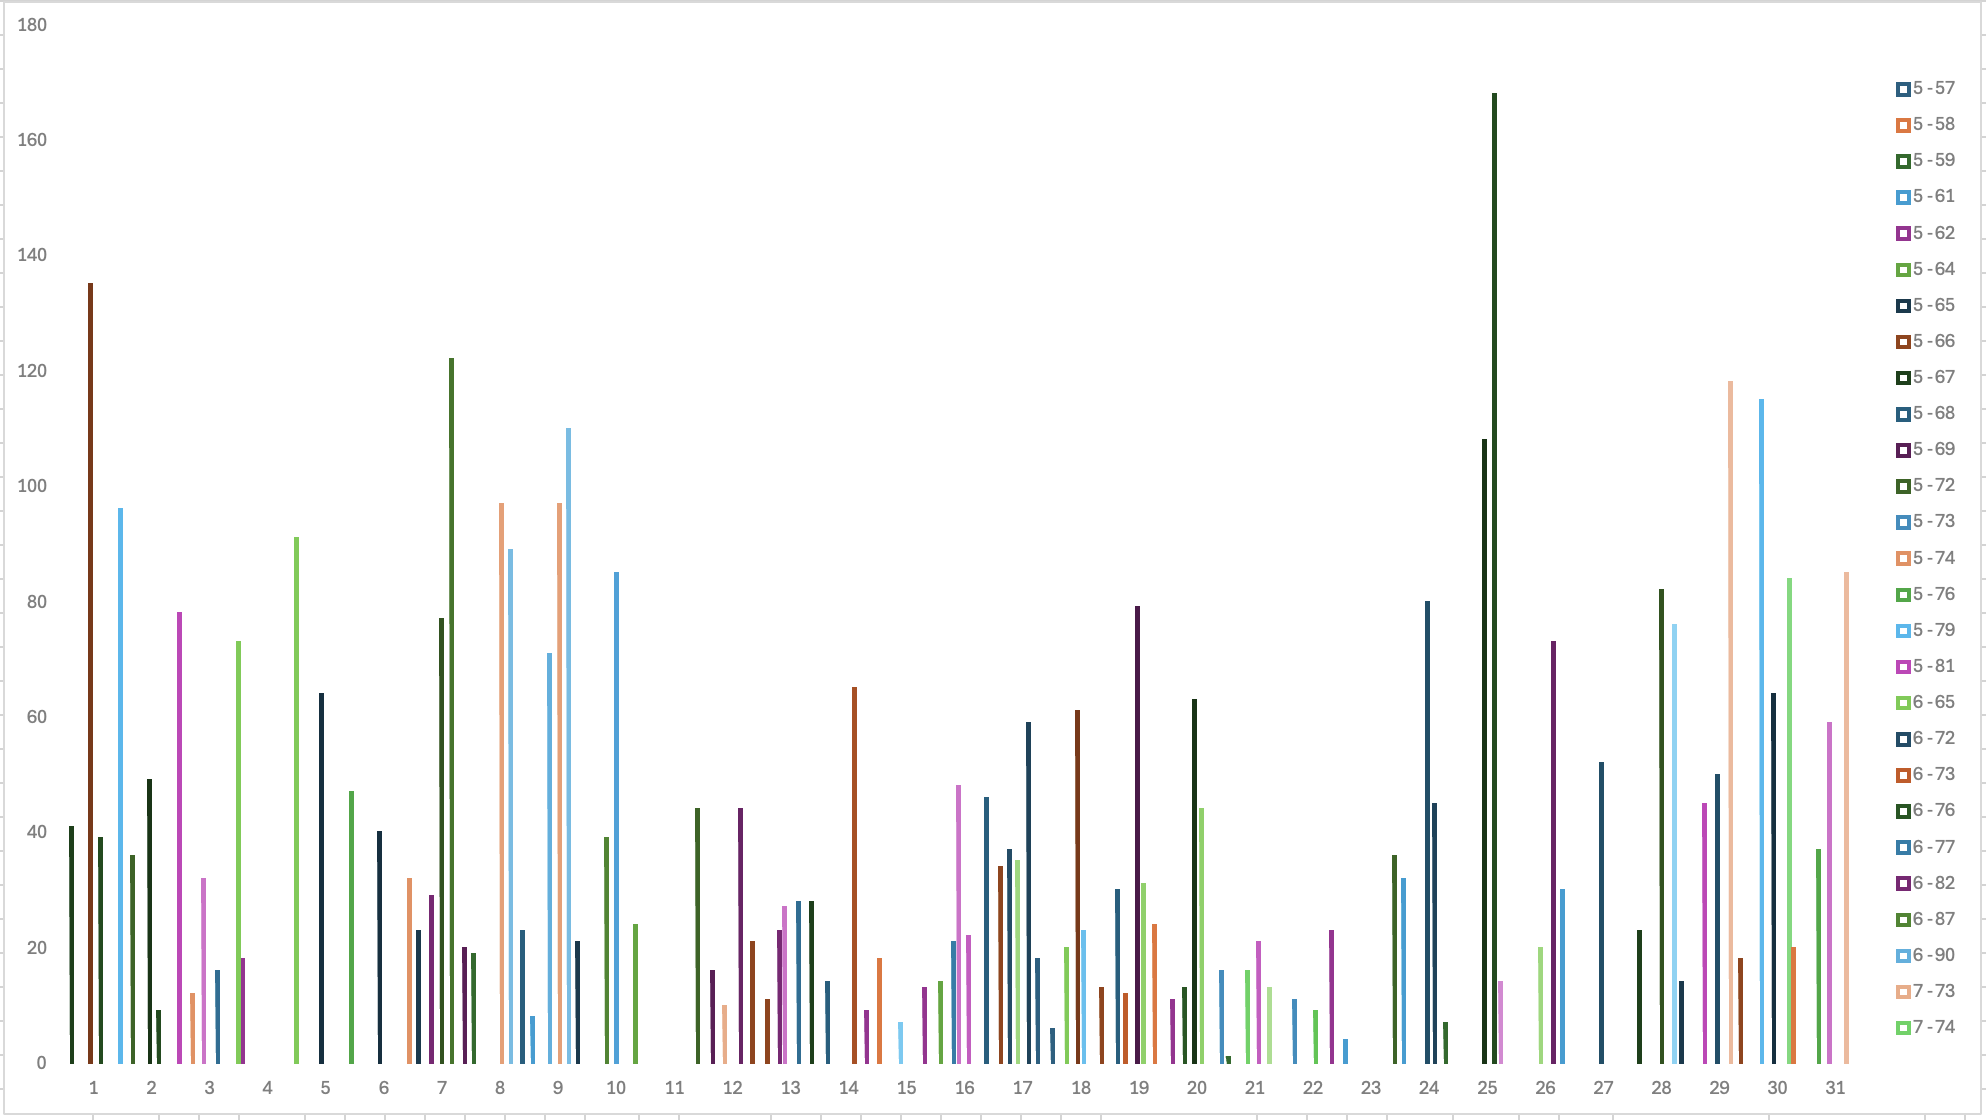
\includegraphics{pivot4_chart_baruga.png}

\textbf{Pivot Table of Variation in Solar Radiation and Temperature}

\begin{itemize}
\tightlist
\item
  The pivot chart provide a visual representation of how these variables
  change over time. The histogram shows day-to-day variations in ozone
  levels, with the highest concentrations occurring in the summer
  months. Notably, there is a pronounced peak around July 25th,
  indicating exceptionally high ozone levels on that day. May and July
  both have elevated levels, with smaller peaks around May 29th and
  30th, but July 25th stands out as the most significant. Overall, the
  chart confirms that ozone levels are highest in July, particularly
  around the 25th.
\end{itemize}

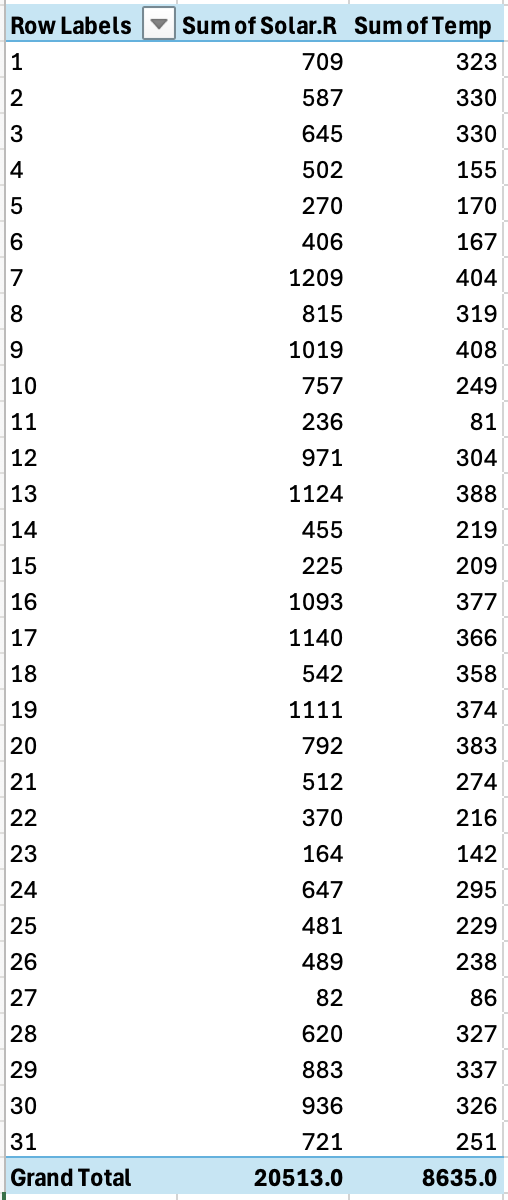
\includegraphics{pivot1_table_baruga.png}

\begin{itemize}
\tightlist
\item
  The pivot table shows daily sums for Solar Radiation and Temperature
  over a month. There is noticeable daily variation, with high values on
  days like 18, 19, and 29, indicating intense sunlight and warmer
  temperatures, and lower values on days like 23 and 27, reflecting
  cooler conditions. The grand totals summarize the entire month, with
  20,513 for Solar Radiation and 8,635 for Temperature. Overall, the
  table captures daily fluctuations in weather conditions.
\end{itemize}

** Pivot Chart of Pivot Chart of Variation in Solar Radiation and
Temperature**

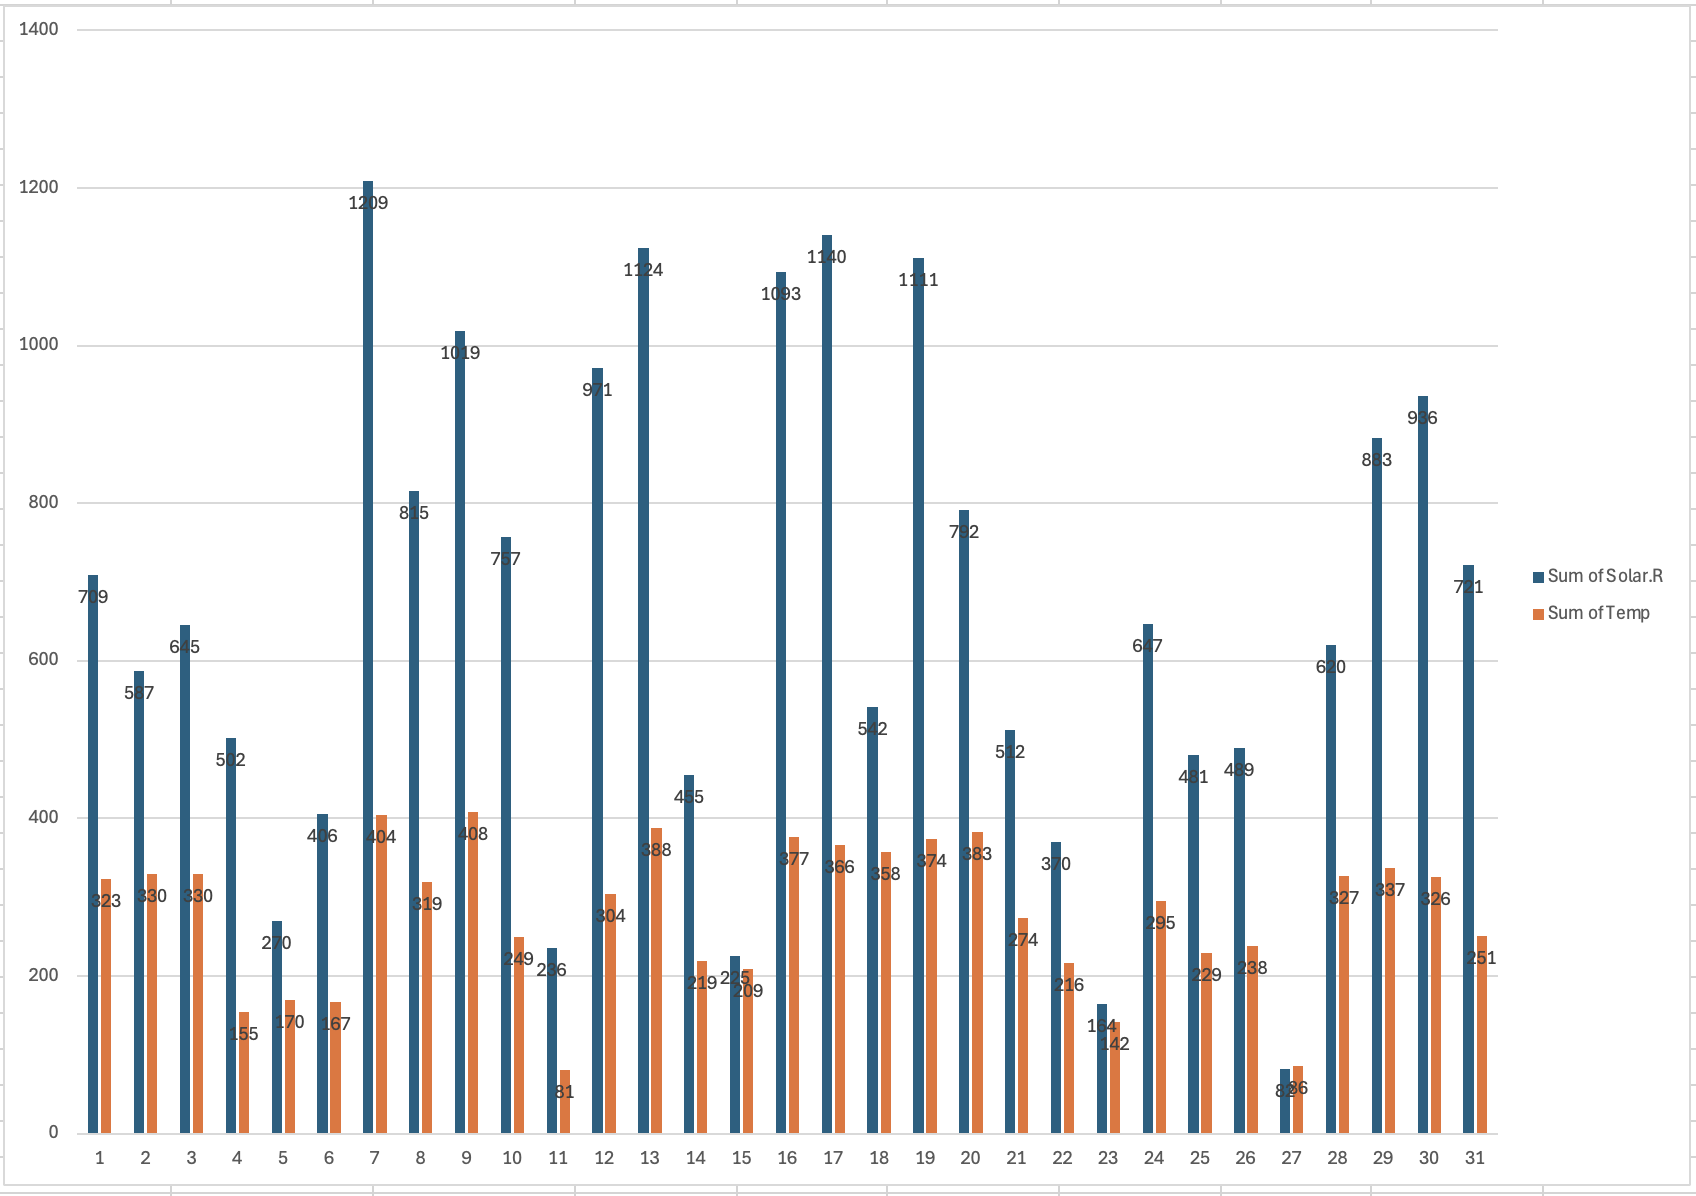
\includegraphics{pivot1_chart_baruga.png}

\begin{itemize}
\tightlist
\item
  The bar chart shows daily sums of Solar Radiation (blue) and
  Temperature (orange) over 31 days. High Solar Radiation is notable on
  days like 9, 13, 16, 18, 19, and 29, with values exceeding 1,000.
  Temperature values are generally lower, mostly below 400, with higher
  values on days like 9 and 18. There are significant day-to-day
  variations, with some days showing high Solar Radiation but lower
  temperatures (e.g., Day 13). The chart captures daily fluctuations and
  highlights days with extreme values.
\end{itemize}

\textbf{Pivot Table}

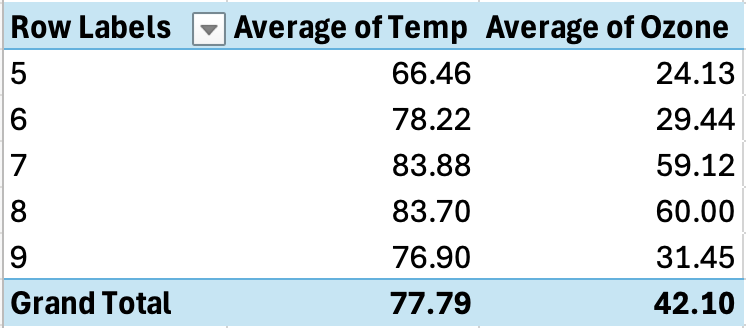
\includegraphics{pivot2_table_baruga.png}

\begin{itemize}
\tightlist
\item
  The pivot table displays the average temperature
  (\texttt{Average\ of\ Temp}) and ozone levels
  (\texttt{Average\ of\ Ozone}) for days labeled 5 to 9, showing average
  temperatures ranging from 66.46 to 83.88, with the highest
  temperatures recorded on days 7 and 8. Ozone levels vary
  significantly, from a low of 24.13 on Day 5 to a high of 60.00 on Day
  8. Overall, the average temperature for the period is 77.79, and the
  average ozone level is 42.10, reflecting moderate temperatures with
  variable ozone levels across these days and highlighting daily
  fluctuations in both metrics.
\end{itemize}

\textbf{Pivot Chart}

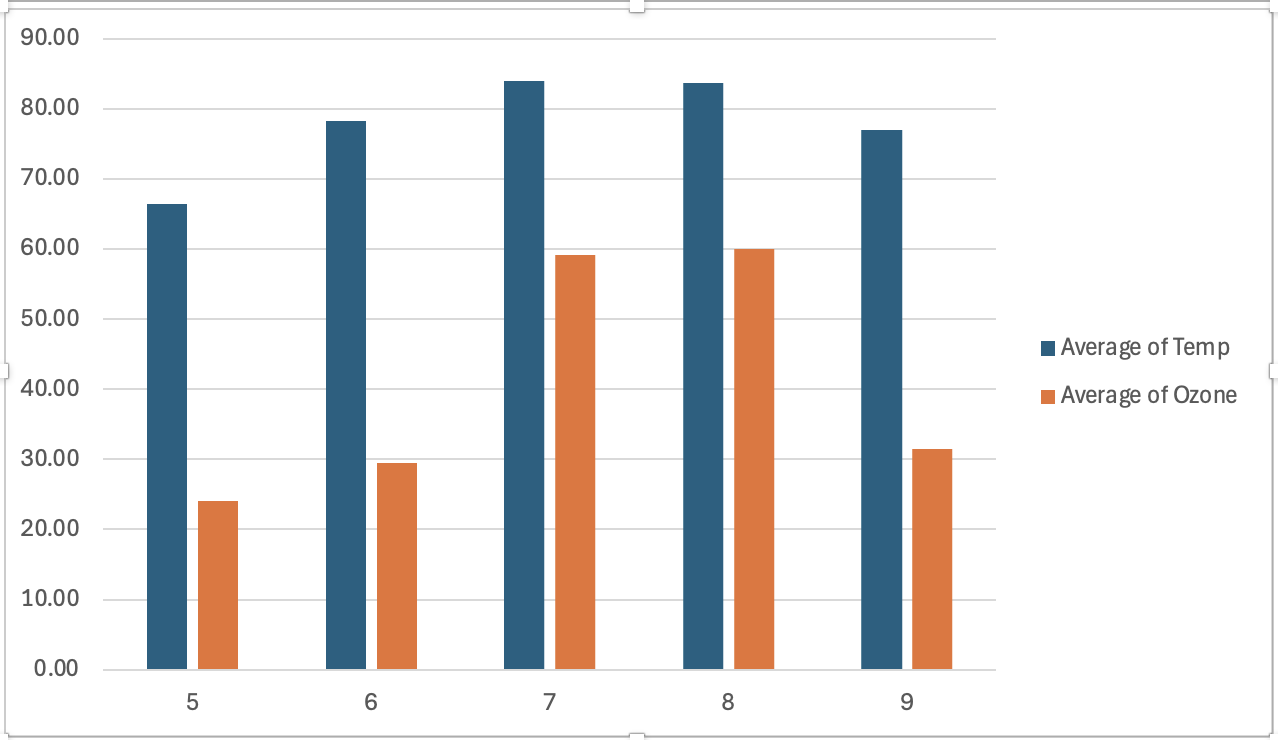
\includegraphics{pivot2_chart_baruga.png}

\begin{itemize}
\tightlist
\item
  The bar chart illustrates the average temperature (in blue) and
  average ozone levels (in orange) for days 5 to 9, showing that
  temperatures remain relatively high throughout, ranging from around 66
  on Day 5 to approximately 84 on Days 7 and 8. Ozone levels start low
  on Day 5 (around 24), rise significantly by Days 7 and 8 (around
  59-60), and then decrease slightly on Day 9 (around 31). The chart
  suggests a potential correlation between higher temperatures and
  elevated ozone levels, as Days 7 and 8, which have the highest
  temperatures, also show the highest average ozone levels, indicating
  noticeable variability over the period.
\end{itemize}

\subsection{Week 3}\label{week-3-5}

\section{Friday}\label{friday-2}

\subsection{Week 1}\label{week-1-7}

\subsection{Week 2}\label{week-2-7}

\subsection{Week 3}\label{week-3-6}

\section{Midterm Project}\label{midterm-project-2}

\subsection{Week 1}\label{week-1-8}

title: ``Midterm\_Project\_Baruga'' subtitle: ``Data.gov: Warehouse and
Retail Sales'' format: html ---

\textbf{Context of the Dataset}

\begin{itemize}
\tightlist
\item
  \textbf{Title}: Warehouse and Retail Sales
\item
  \textbf{Link}:
  \href{https://data.montgomerycountymd.gov/api/views/v76h-r7br/rows.csv?accessType=DOWNLOAD}{Download
  the CSV dataset}
\end{itemize}

The \emph{Warehouse and Retail Sales} dataset provides a comprehensive
view of sales activities in Montgomery County, Maryland, by capturing
data from various warehouse and retail operations. This dataset was
collected through a combination of direct reporting from businesses,
automated sales tracking systems, and regional sales surveys. The data
encompasses a range of sales metrics, including volume and product
categories, to offer insights into business performance across different
types of establishments.

The dataset includes the following variables:

\begin{itemize}
\tightlist
\item
  Row Labels: Categories or identifiers used to organize and classify
  the sales data.
\item
  BEER: Sales volume for beer products.
\item
  DUNNAGE: Sales volume for dunnage products, which are materials used
  to protect goods during transportation.
\item
  KEGS: Sales volume for kegs, typically used for storing and
  transporting beverages.
\item
  LIQUOR: Sales volume for liquor products.
\item
  NON-ALCOHOL: Sales volume for non-alcoholic beverages.
\item
  REF: Sales volume for refrigeration supplies or products.
\item
  STR\_SUPPLIES: Sales volume for store supplies, which may include
  various retail essentials.
\item
  WINE: Sales volume for wine products.
\item
  Grand Total: The total sales volume across all categories combined.
\end{itemize}

** Data Cleaning and Preparation**

\begin{enumerate}
\def\labelenumi{\arabic{enumi}.}
\tightlist
\item
  \textbf{Import the Data}: I downloaded and loaded the CSV file into
  Excel.
\item
  \textbf{Check for Missing Values}: My preferred method for handling
  NAs is by highlighting them and deselecting them using the filter tool
  for each column as I feel most thorough by doing that. Using the
  following steps ``Select the entire dataset, go to Home \textgreater{}
  Conditional Formatting \textgreater{} Highlight Cells Rules
  \textgreater{} Blanks to highlight all blank cells.''
\item
  \textbf{Data Formatting}: Formated any columns that need specific data
  types (such as dates as date format, numbers as currency or
  percentage).
\end{enumerate}

\begin{itemize}
\tightlist
\item
  Specifically I used the =TEXTJOIN(``-'', TRUE, A2, B2) function to
  join column one (YYYY) and column two (MM) into a new column called
  TIME
\end{itemize}

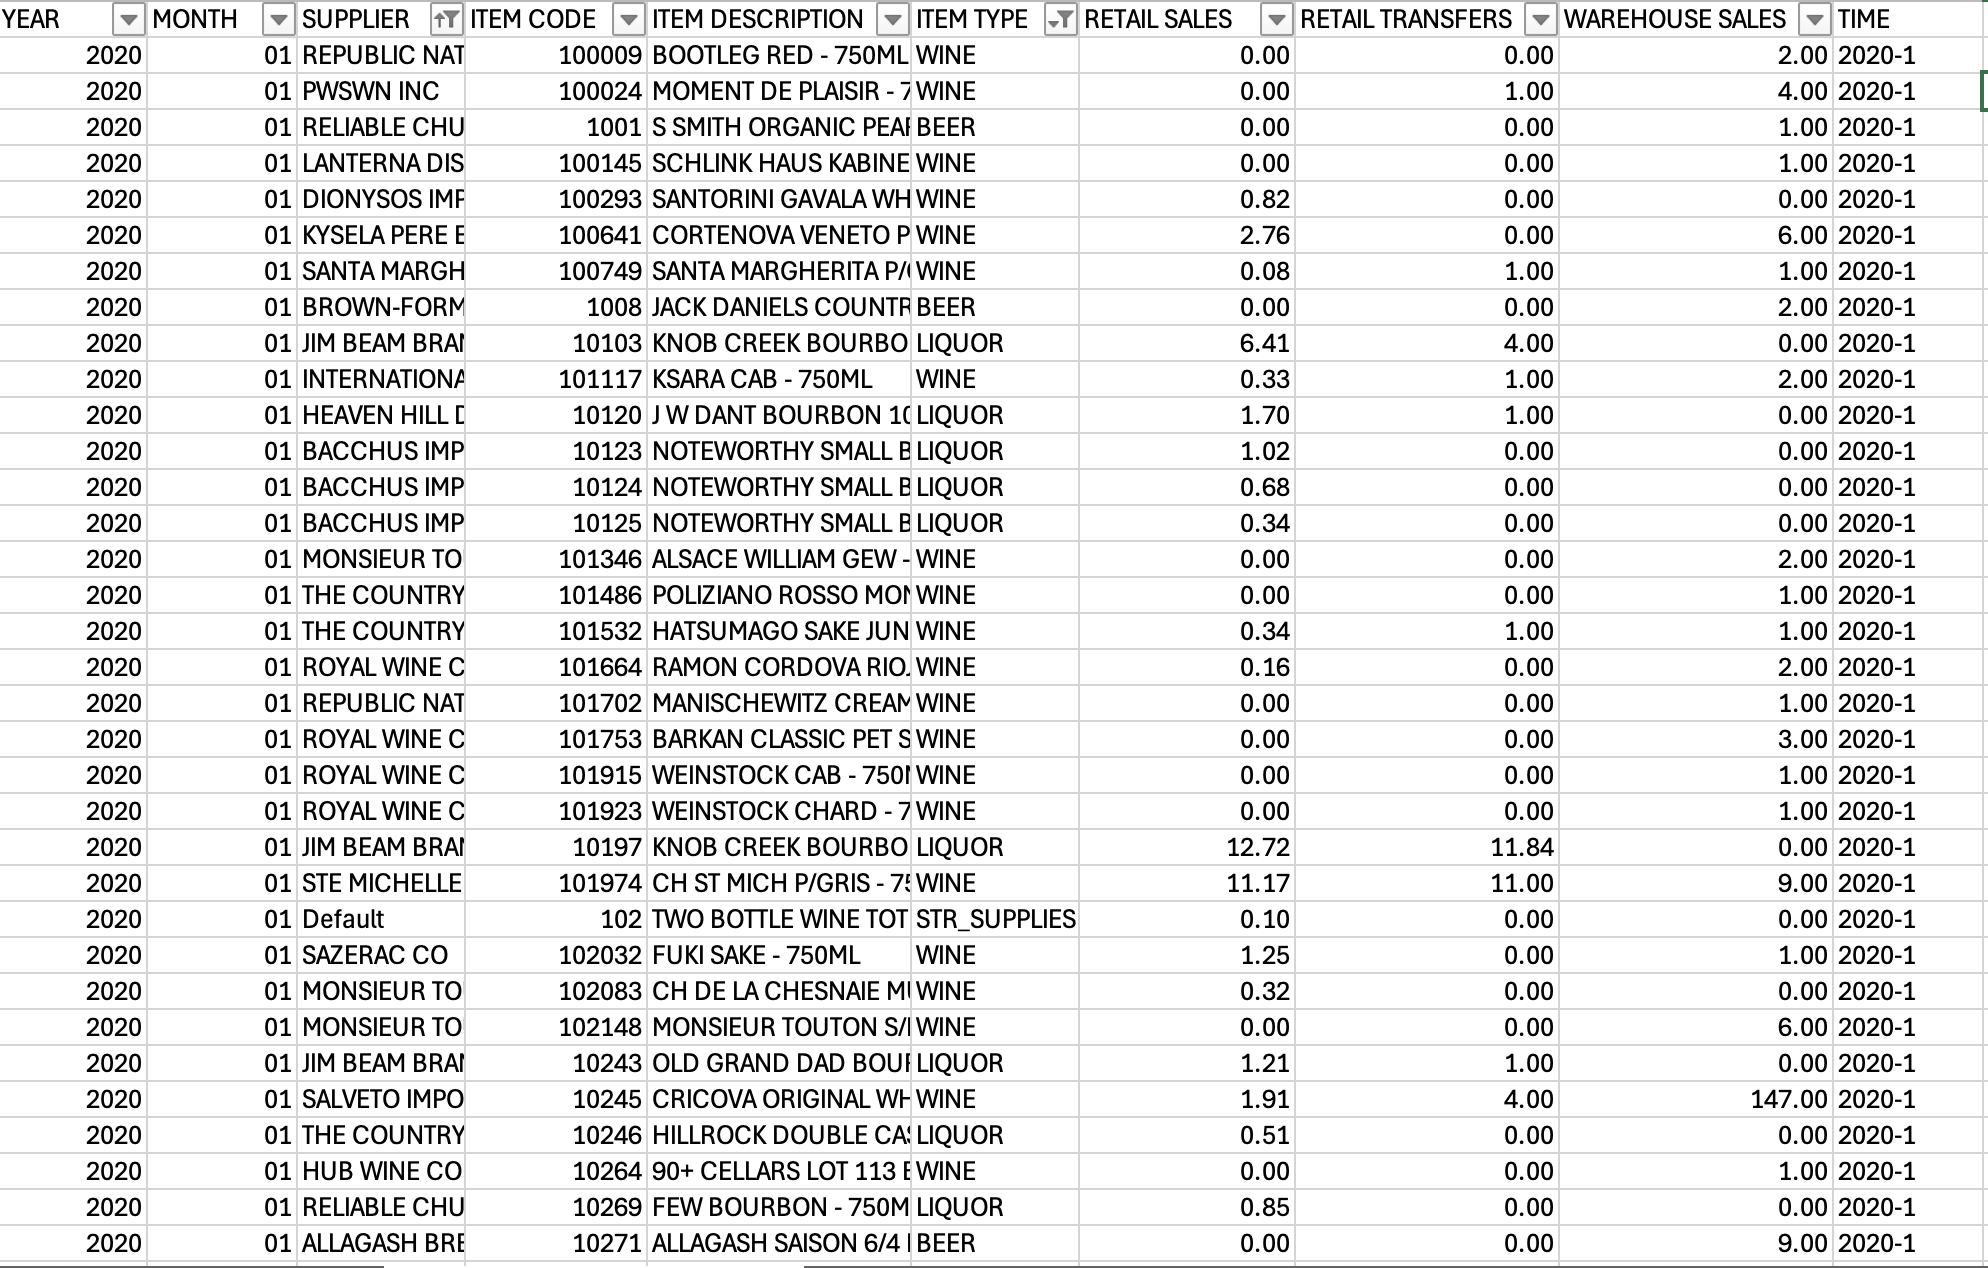
\includegraphics{summary_screenshot.png}

\textbf{Visualization}

\textbf{Pivot Tables YT link:}
https://www.youtube.com/watch?v=qu-AK0Hv0b4

\begin{itemize}
\tightlist
\item
  Pivot tables are a powerful and user friendly (drag and drop) summary
  statistic/visualisation tool that I used to get an intial feel of my
  data.
\end{itemize}

Here are the findings:

\textbf{Warehouse Sales/Expenses of Beverages Over Time (2017 - 2020)}

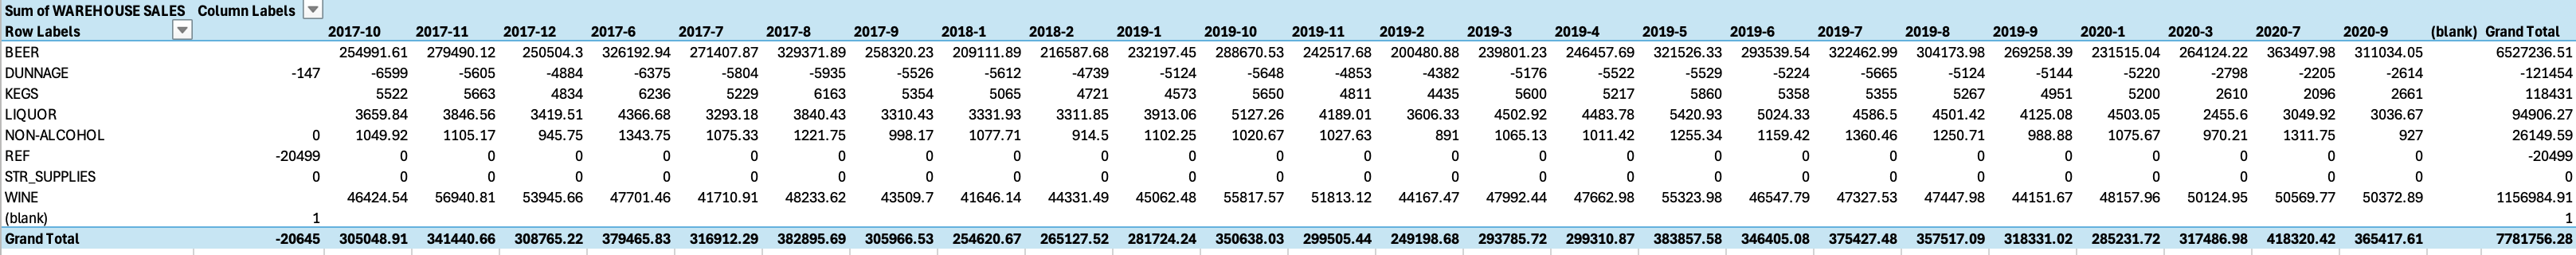
\includegraphics{pivot_table_baruga.png}

\begin{itemize}
\tightlist
\item
  \textbf{Overall Sales}: \textbf{\emph{BEER}} has the highest sales,
  followed by \textbf{\emph{WINE}}, while \textbf{\emph{DUNNAGE}},
  \textbf{\emph{REF}}, and \textbf{\emph{STR\_SUPPLIES}} have negative
  or minimal sales, which makes sense as refers to materials used to
  protect goods during shipping and handling, such as packing materials
  or cushioning, and as such is an expense to the business leading to
  its negative output on revenue.
\item
  \textbf{Monthly Trends}: \textbf{\emph{BEER}} sales vary
  significantly, with large peaks and drops. \textbf{\emph{WINE}} sales
  are more stable but still show some fluctuation. \textbf{\emph{KEGS}}
  and \textbf{\emph{LIQUOR}} show positive but lower sales.
\end{itemize}

\textbf{Histogram of Warehouse Sales/Expenses of Beverages Over Time}

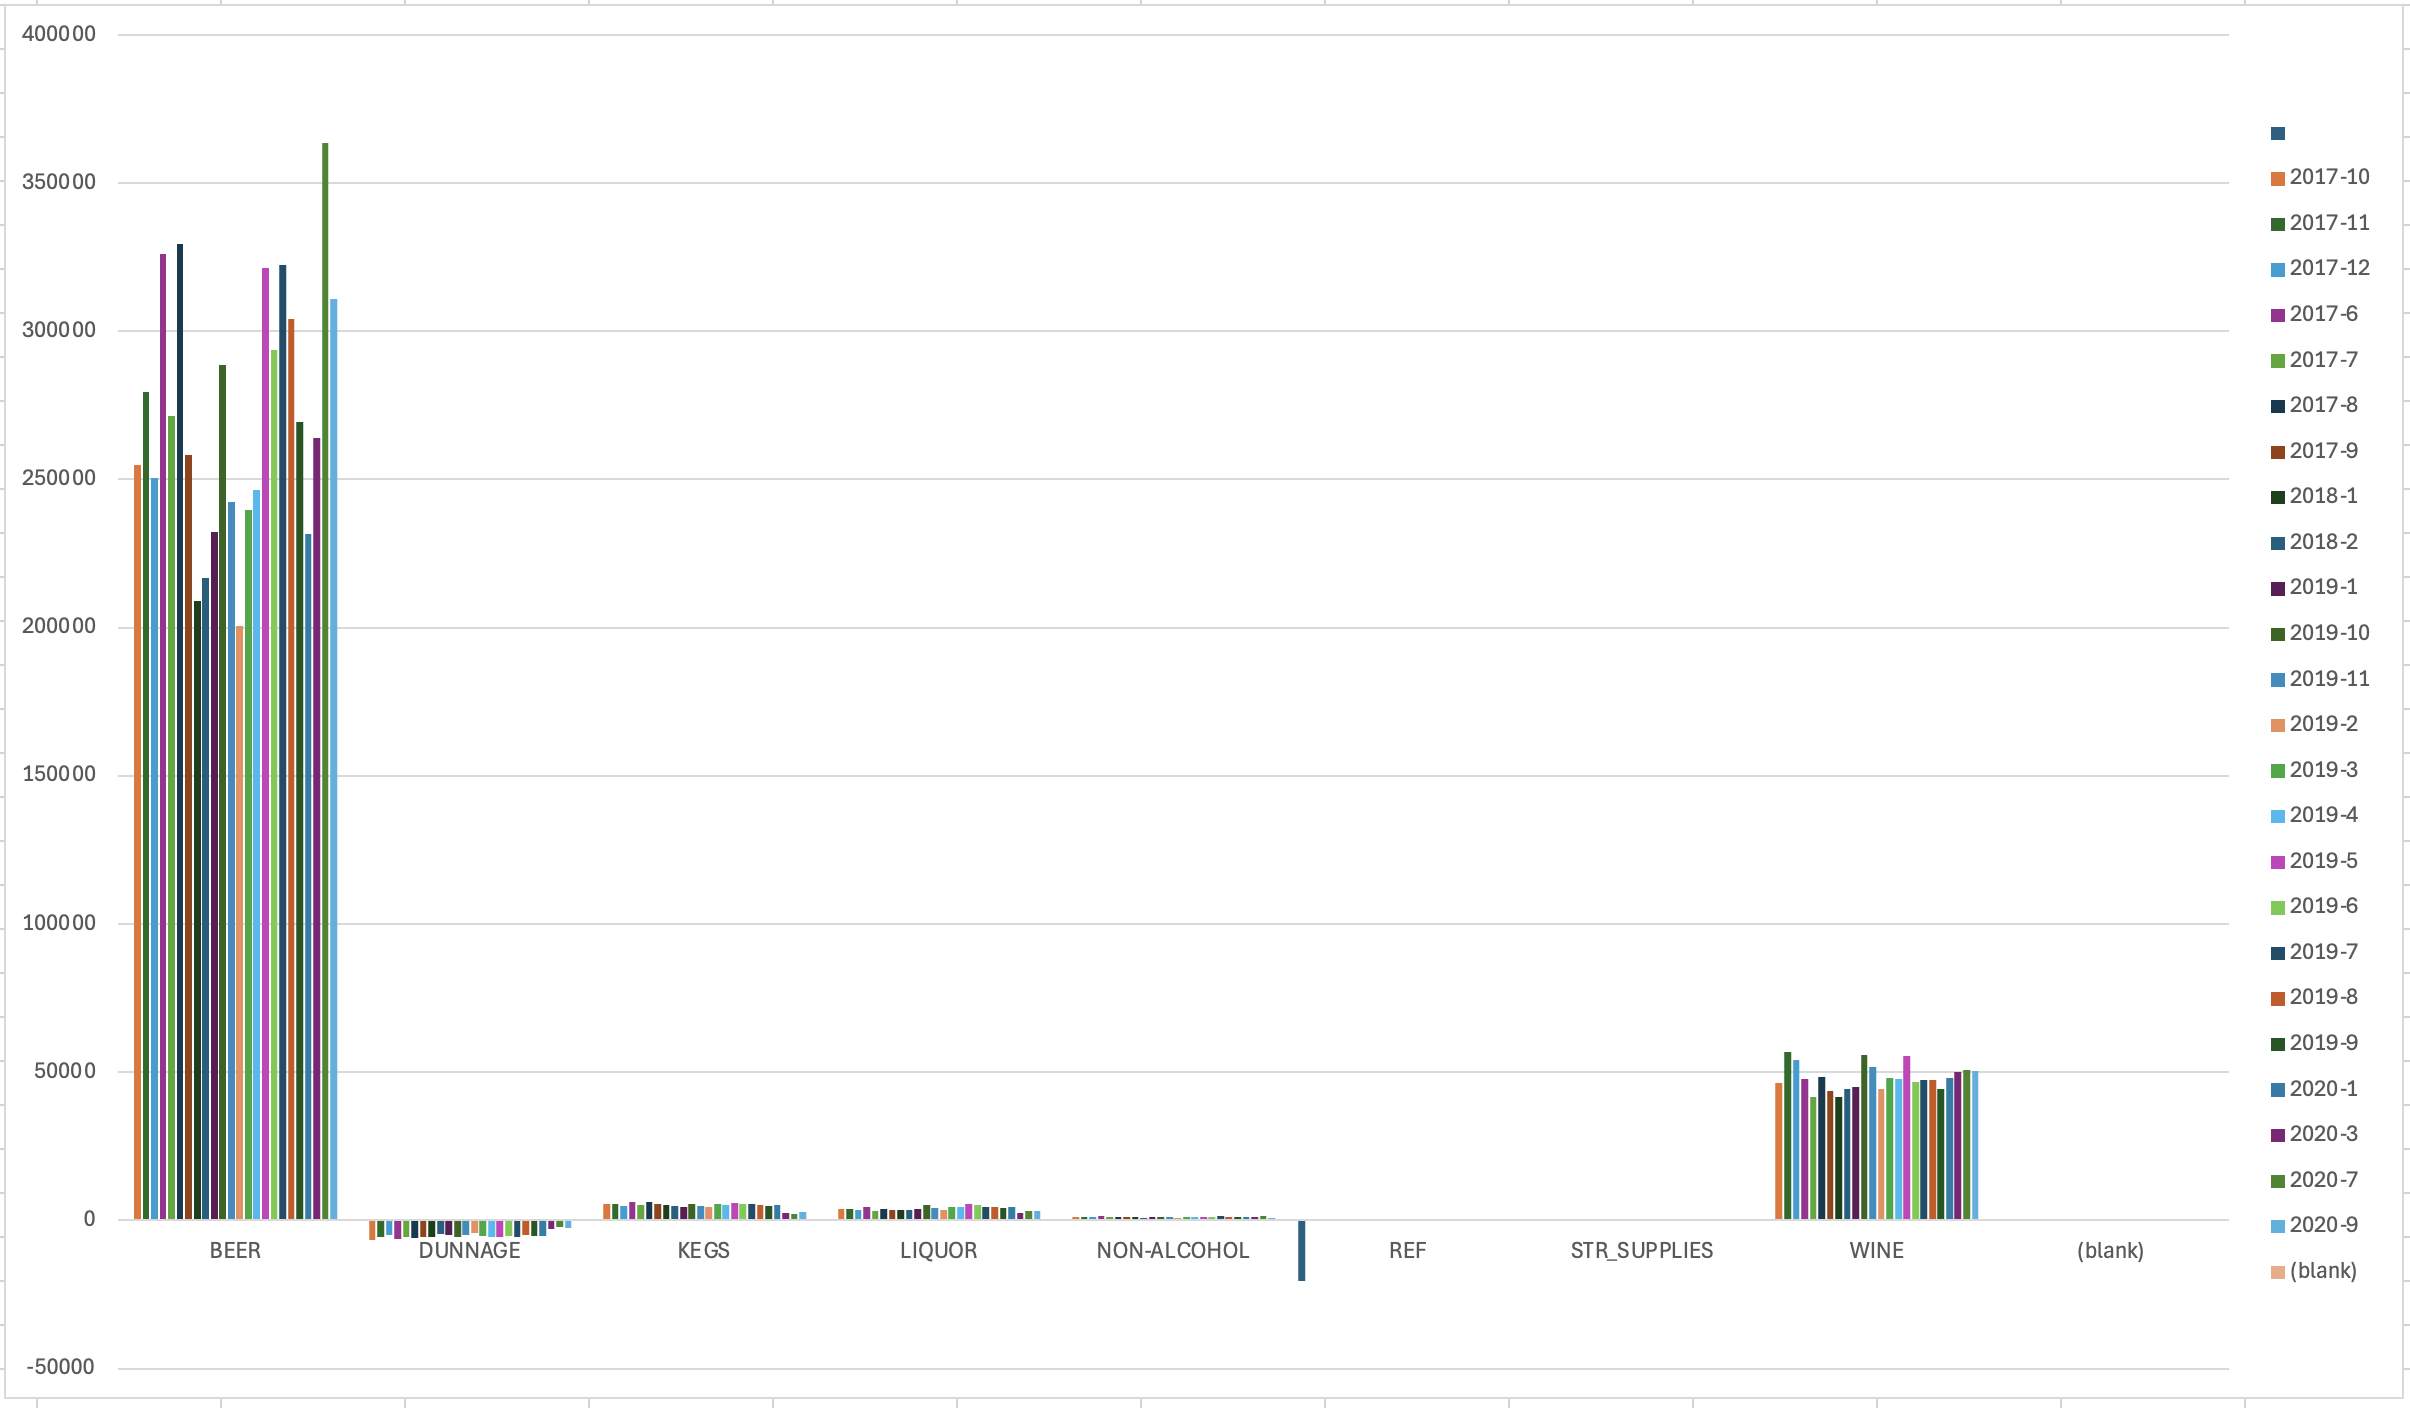
\includegraphics{pivot_chart.png}

\begin{itemize}
\tightlist
\item
  Here is a histogram representation of the aforementioned summary pivot
  tables. There appears to be a disporportionate amount of
  \textbf{\emph{BEER}} bought for warehouses. But that could be due to
  the fact that beers are sold in packs and so single unit quantity has
  skyrocketed in order to make a ``12 pack'' that will later count as
  one unit sold at retail.
\end{itemize}

\textbf{Retail Sales of Beverages Over Time (2017 - 2020)}

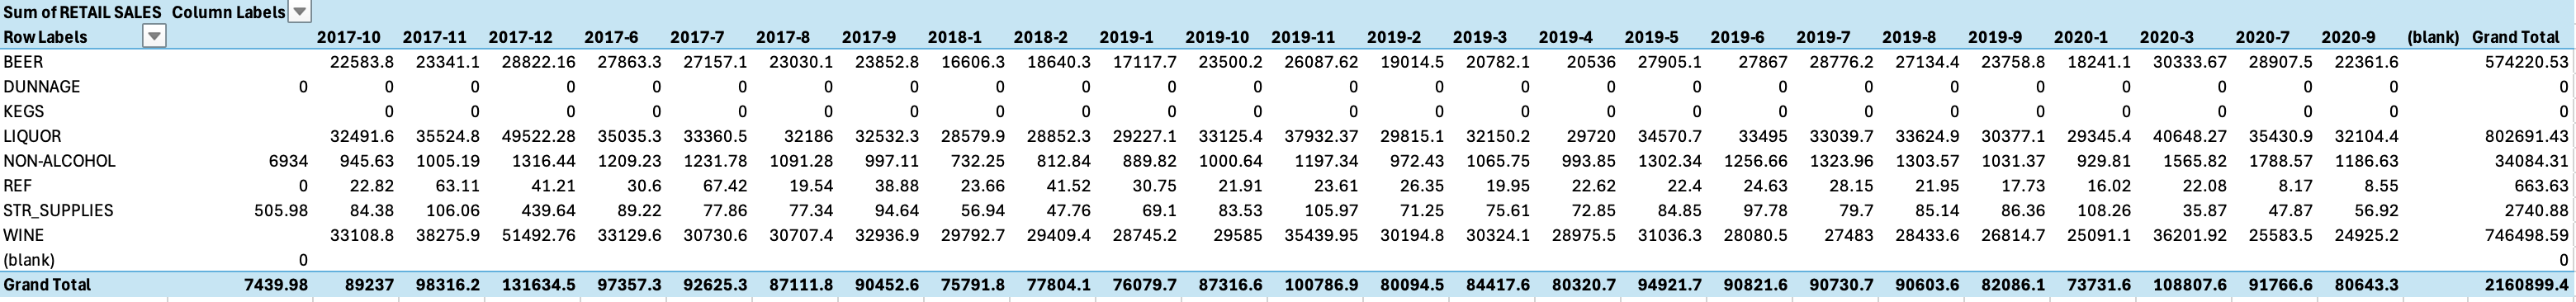
\includegraphics{pivot2_table.png}

\begin{itemize}
\tightlist
\item
  \textbf{Product Types}: Includes Beer, Liquor, Wine, Non-Alcoholic
  beverages, and others, with substantial sales figures for Beer,
  Liquor, and Wine.
\item
  \textbf{Sales Trends}: Liquor leads with \$802,691.43 in total sales,
  followed by Wine (\$746,498.59) and Beer (\$574,220.53). Recent months
  show higher sales for Beer and Wine.
\item
  \textbf{Low Sales Categories}: Items like Dunnage and Kegs have
  negligible or zero sales.
\item
  \textbf{Overall Total}: Total sales across all products amount to
  \$2,160,899.37, highlighting overall retail activity.
\end{itemize}

\textbf{Histogram of Retail Sales of Beverages Over Time}

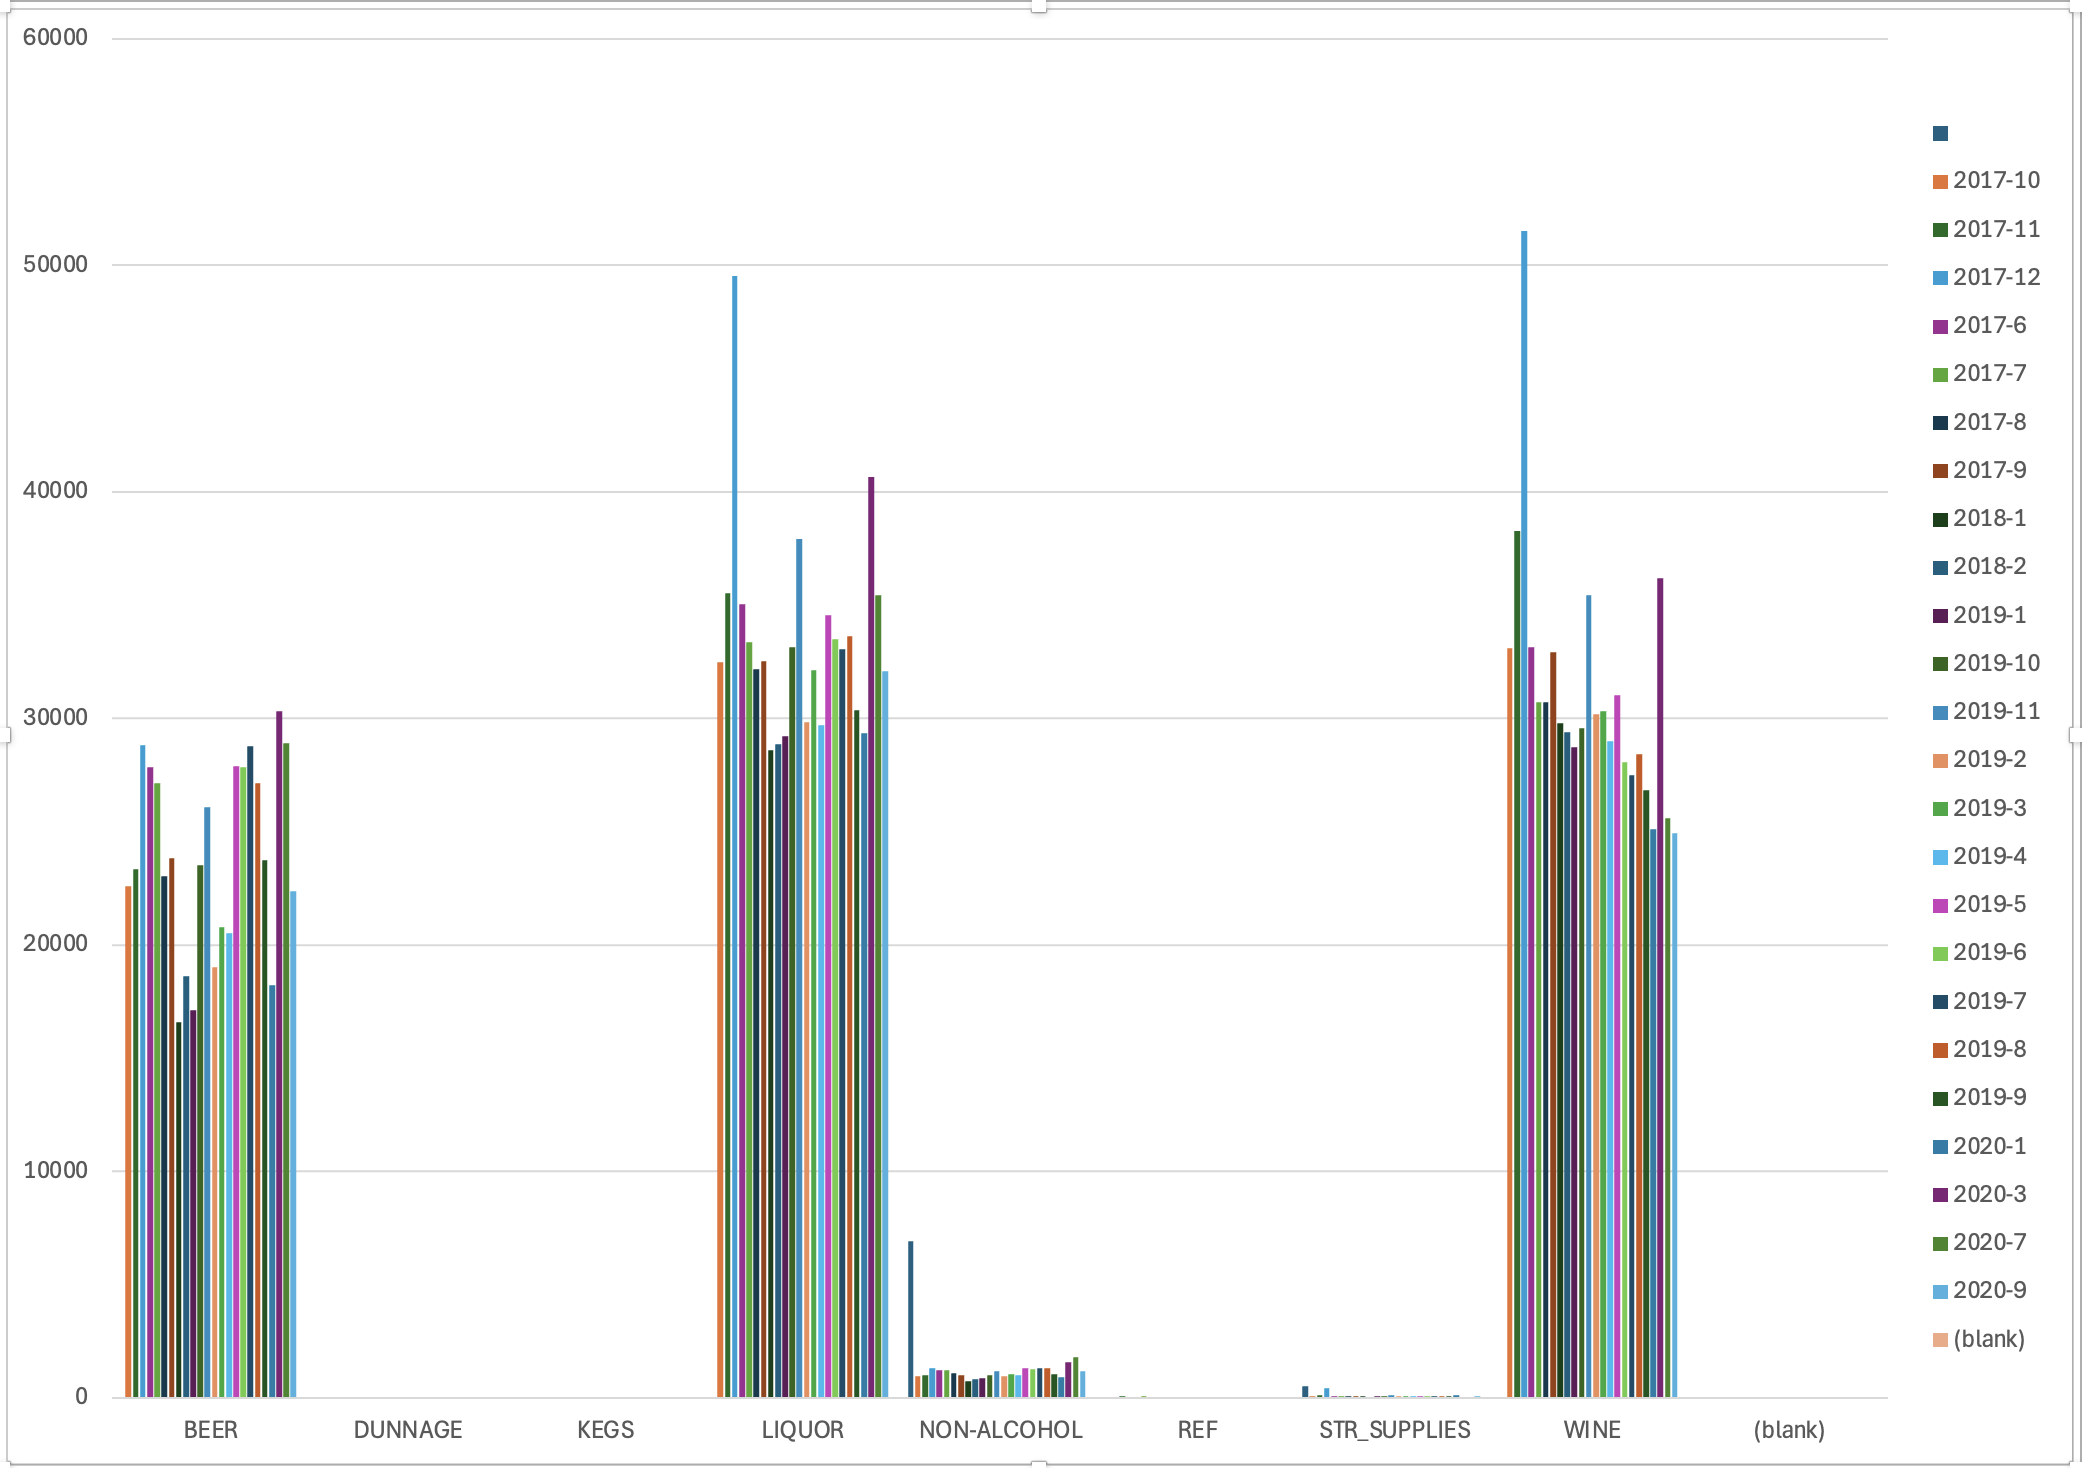
\includegraphics{pivot_chart_2.png}

\begin{itemize}
\tightlist
\item
  Once we come to the retail side of things we see that
  \textbf{\emph{WINE}} and \textbf{\emph{LIQUOR}} are clear best
  sellers. It is shown hower that \textbf{\emph{LIQUOR}} has begun to
  overtake \textbf{\emph{WINE}} in retail sales.
\end{itemize}

** Summary**

From the ``Warehouse and Retail Sales'' dataset, I found that Beer leads
in warehouse sales, with notable fluctuations due to bulk packaging,
while Wine and Liquor have more stable sales. Retail sales show Liquor
as the top seller, recently surpassing Wine, with Beer also performing
strongly but declining. The histograms illustrate high Beer volume in
warehouses and a shift in retail dominance from Wine to Liquor. Next, I
will analyze seasonal trends, create advanced visualizations for deeper
insights, and finalize the report with comprehensive findings and
recommendations. \#\#\# Week 2 \#\#\# Week 3

\subsection{Week 2}\label{week-2-8}

\subsection{Week 3}\label{week-3-7}

\bookmarksetup{startatroot}

\chapter{Toluwanimi Olufawo}\label{toluwanimi-olufawo}

This page contains all of Toluwanimi Olufawo submissions this semester
organized into different sections.

\section{Wednesday}\label{wednesday-3}

\subsection{Week 1}\label{week-1-9}

\subsection{Week 2}\label{week-2-9}

Click to expand Week 2

I am using the air-quality dataset, which contains air quality
measurements collected from May to September. This dataset includes:

\begin{itemize}
\tightlist
\item
  \textbf{Ozone}
\item
  \textbf{Solar.R} (solar radiation)
\item
  \textbf{Wind} (wind speed in mph)
\item
  \textbf{Temp} (temperature in Fahrenheit)
\item
  \textbf{Month} (May to September)
\item
  \textbf{Day} (1 to 31)
\end{itemize}

\textbf{Data Cleaning Process}

I cleaned the dataset using Excel by removing rows with missing values
(NA) and performed exploratory analysis to reveal patterns and trends in
ozone levels and other variables.

\textbf{Ozone Histogram}

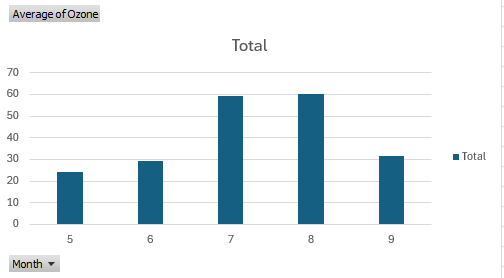
\includegraphics{hist_ozone_toluwanimi.png}

The Ozone distribution shows a right-skewed pattern, indicating that
most values are low, with a few high outliers. This could reflect
variations in weather or pollution.

\textbf{Scatter Plot: Ozone vs Temperature}

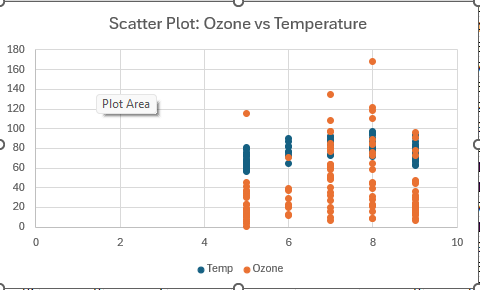
\includegraphics{scatter_ozone_vs_temp_toluwanimi.png}

There is a weak positive correlation between ozone and temperature,
suggesting that higher temperatures tend to coincide with higher ozone
levels, though other factors like wind or pollution likely contribute.

\textbf{Average Ozone Per Day \& Month}

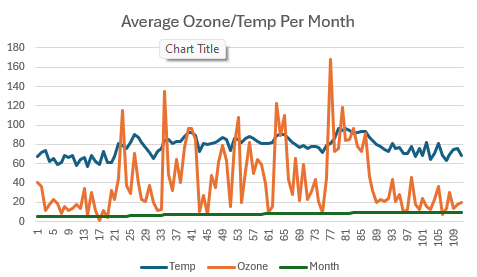
\includegraphics{pivot4_table_toluwanimi.png}

The highest ozone averages occur on May 25th and July 25th, with notable
peaks also on May 29th and July 30th. July generally exhibits higher
ozone levels, especially around the end of the month.

\textbf{Solar Radiation and Temperature Variations}

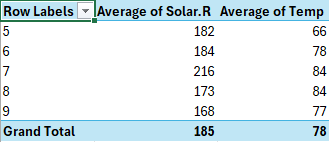
\includegraphics{pivot1_chart_toluwanimi.png}

The chart reveals daily variations in solar radiation and temperature,
peaking around days 18, 19, and 29. Both solar radiation and temperature
are higher on these days, pointing to intense sunlight and warmth during
these periods.

\textbf{Daily Averages of Temperature and Ozone}

\includegraphics{pivot2_chart_toluwanimi.png}

Ozone levels peak on days 7 and 8, correlating with higher temperatures,
showing that warmer days generally have higher ozone values, although
this trend doesn't apply across all days.

\subsection{Week 3}\label{week-3-8}

\section{Friday}\label{friday-3}

\subsection{Week 1}\label{week-1-10}

\subsection{Week 2}\label{week-2-10}

\subsection{Week 3}\label{week-3-9}

\section{Midterm Project}\label{midterm-project-3}

\subsection{Week 1}\label{week-1-11}

\subsection{Week 2}\label{week-2-11}

\subsection{Week 3}\label{week-3-10}

\href{introduction.html}{Back to Main Page}

\bookmarksetup{startatroot}

\chapter{Summary}\label{summary}

In summary, this book has no content whatsoever.

\begin{Shaded}
\begin{Highlighting}[]
\DecValTok{1} \SpecialCharTok{+} \DecValTok{1}
\end{Highlighting}
\end{Shaded}

\begin{verbatim}
[1] 2
\end{verbatim}

\bookmarksetup{startatroot}

\chapter*{References}\label{references}
\addcontentsline{toc}{chapter}{References}

\markboth{References}{References}

\phantomsection\label{refs}
\begin{CSLReferences}{0}{1}
\end{CSLReferences}



\end{document}
